\documentclass[11pt,a4paper]{article}
\usepackage[margin=22mm]{geometry}
\usepackage{graphicx,booktabs,amsmath,hyperref,tabularx,array,float}
\hypersetup{colorlinks=true,urlcolor=blue,linkcolor=blue}
\sloppy
\setlength{\parindent}{0pt}\setlength{\parskip}{6pt}
\newcommand{\uv}{\ensuremath{\mu\mathrm{V}}}
\title{Input contamination in the ErrP pilot dataset\\\large An input-only screening research note}
\author{Satyam Awasthi}\date{}
\begin{document}\maketitle
\begin{abstract}
We screened all eligible movement-centred input intervals from two pilot participants, before FORCe or the final low-pass. The inventory covers 29 recordings, 2,799 trials, 8,397 one-second windows and 67,176 channel-window measurements. Gross excursions exceeding 1 mV occurred in 180 of 1,411 mle01 trials and none of 1,388 spe30 trials. Further relative spectral and morphological outliers warrant inspection. These observations support data-quality handling, but do not establish artifact-source identities, the necessity of FORCe, or successful artifact removal. Input-only examples are provided for expert review.
\end{abstract}
\section{Question and scope}
The first question is whether the inputs contain contamination that could compromise analysis. This report addresses its measured indicators and review examples. It does not compare cleaners, estimate EOG/EMG sensitivity, or assess classification. The two participants provide positive evidence that the dataset contains problematic recordings; they cannot establish prevalence across the remaining participants. An absence of flags would not prove clean EEG.

All eight recorded EEG channels are included: P3, PO3, PO7, CP5, CP1, Cz, FCz and FC1. There are no independent EOG/EMG channels and no frontopolar electrodes in this montage. Therefore suspected ocular and muscle activity remain hypotheses. A transient visual response is neural activity and is considered separately as a possible task-related confound, rather than automatically an artifact.
\section{Input and measurement methods}
\subsection{Input preprocessing and inclusion}
The sampling rate is 500 Hz, and recorded EEG values are converted from nanovolts to microvolts. The input $x$ is continuously filtered with a fourth-order Butterworth 1 Hz high-pass using forward-backward filtering, before trial extraction.

This pilot includes intervals with an available movement marker and a complete valid three-second segment after gap and recording-edge checks. These are this analysis's input-inclusion checks, not eligibility criteria attributed to the paper. Of 2,915 trial rows, 116 fail these checks and 2,799 remain. Inclusion does not apply the production pipeline's final amplitude rejection.

Each interval spans $[-1.5,1.5)$ s relative to movement onset (marker 400). Measurements use three separate one-second windows: $[-1.5,-0.5)$, $[-0.5,0.5)$ and $[0.5,1.5)$. Differences never cross these window boundaries. No FORCe, low-pass, trial baseline correction or new rereferencing is applied to the measured input. Raw traces provide context for slow shifts. Display-only centring does not change the measurements.
\subsection{Exploratory screens}
One-sided power spectral density (PSD) estimates are obtained from demeaned one-second windows using a periodic Hann window and a periodogram. Frequency spacing is $\Delta f=1$ Hz. One band RMS value is computed for each channel and window:
\[
f_{\mathrm{band},i}=\sqrt{\sum_{k\in\mathrm{band}}\mathrm{PSD}_i[k]\,\Delta f}.
\]
The slow band is 1--4 Hz; the higher-frequency band is 30--90 Hz excluding 48--52 Hz. Power near 50 Hz is inspected separately. The local abrupt feature is the largest absolute adjacent-sample change within one window:
\[
f_{\mathrm{step},i}=\max_{n=2,\ldots,500}|x_i[n]-x_i[n-1]|.
\]

Potential outliers were flagged using a modified z-score based on the median absolute deviation (MAD), calculated on log-transformed feature values. Scores above 3.5 were flagged for inspection, rather than classified automatically as artifacts:
\[
z_{f,i}=0.67448975\frac{\log_{10}(f_i)-\operatorname{median}_j(\log_{10}f_j)}{\operatorname{MAD}_j(\log_{10}f_j)},\qquad
\operatorname{MAD}(v)=\operatorname{median}_j|v_j-\operatorname{median}(v)|.
\]
The score is applied separately to slow-band RMS, higher-frequency RMS and the step feature. Each feature was scored relative to its values across trials from the same participant, session, channel and one-second window position. Persistent contamination within a group can be missed or can distort its reference distribution.

The NIST handbook describes the modified z-score and an absolute-score threshold of 3.5 for potential outliers \cite{nist}. Here only the upper tail ($z_f>3.5$) is screened for unusually large features. The threshold is used descriptively; it is not an EEG-specific artifact cut-off or a significance test.

Table~\ref{tab:screens} defines the screens and possible interpretations. A window may meet multiple screening criteria, so flag counts cannot be summed to obtain the number of distinct flagged windows. Likewise, a trial can meet more than one criterion; trial counts cannot be summed to obtain distinct flagged trials. A trial is flagged when any of its channel-windows meets the rule. These screens do not automatically reject a trial.

\begin{table}[H]\centering\small
\renewcommand{\arraystretch}{1.15}
\begin{tabularx}{\linewidth}{@{}p{.18\linewidth}p{.34\linewidth}X@{}}\toprule
Flag/screen & What it detects & What it could indicate\\\midrule
Slow-feature & 1--4 Hz RMS with $z_f>3.5$ & Blinks, eye movements, electrode drift or movement-related contamination; genuine slow EEG activity can also contribute.\\[4pt]
Higher-frequency & 30--90 Hz RMS with $z_f>3.5$, excluding 48--52 Hz & Muscle activity, electrical noise or sharp transients; it does not establish EMG contamination by itself.\\[4pt]
Local abrupt & Step feature with $z_f>3.5$ and channel range $\geq3$ times the median range across channels in that window & Electrode pop, intermittent contact or another channel-local disturbance. The spatial requirement favours local over shared changes.\\[4pt]
Amplitude & Absolute high-pass voltage $>100$ \uv & Large deflection potentially related to ocular activity, movement or electrode problems; an inspection threshold, not automatic rejection.\\[4pt]
Line-frequency & 49--51 Hz power $>25\%$ of 1--90 Hz power & Possible 50 Hz mains interference. A high fraction can also occur when power elsewhere is low.\\[4pt]
Gross excursion & Absolute high-pass voltage $>1$ mV in the three-second interval & Large disturbance warranting recording-quality review; potentially electrode/contact or acquisition problems.\\\bottomrule
\end{tabularx}
\caption{Exploratory input screens and possible sources. Source labels are hypotheses, not independently confirmed identifications.}\label{tab:screens}
\end{table}

A flagged window is counted as overlapping the response interval if it intersects 0.4--0.8 s after movement, the main interval reported in the Graz study \cite{graz}. This overlap is examined because contamination there could affect our ERP analysis. It is a coarse window-level indicator, not evidence that the abnormal samples occur exactly within the response interval.
\subsection{Review selection}
One eligible trial is sampled uniformly from each recording using fixed seed 20261011, giving 29 representative examples. Six additional examples are selected for gross excursions, higher-frequency features, slow deflections and line-frequency content. Enriched examples illustrate possible problems; they cannot estimate prevalence. Informal expert review is pending. Initial assessment should use inputs alone, before displaying cleaning decisions or outputs.
\section{All-trial screening results}
\begin{table}[H]\centering\small
\begin{tabular}{llrrrrr}\toprule
Participant & Session & Eligible & $>1$ mV & Slow & HF & Local\\\midrule
mle01 & pre & 485 & 0 & 7 & 0 & 3 \\
mle01 & post & 478 & 123 & 133 & 104 & 118 \\
mle01 & retest & 448 & 57 & 85 & 45 & 53 \\
spe30 & pre & 495 & 0 & 3 & 3 & 0 \\
spe30 & post & 498 & 0 & 4 & 3 & 0 \\
spe30 & retest & 395 & 0 & 2 & 26 & 0 \\
\bottomrule\end{tabular}
\caption{Trial counts by session. Slow, HF and Local denote exploratory feature flags, not independently confirmed ocular, muscle or electrode artifacts. Counts overlap.}\end{table}

In mle01, 180/1,411 trials (12.8\%) contain a gross excursion: 123 in post and 57 in retest. The largest high-pass input amplitude is approximately 214 mV, in P3 during post run 3, trial 72. Its raw counterpart and large channel-local disturbance support a recording-quality concern, not a routine physiological EEG interpretation. Broad spectral power in these inputs should not be labelled EMG solely from its frequency content.

The amplitude screen flags 258 mle01 trials and 69 spe30 trials. The line-frequency screen flags 41 mle01 trials and no spe30 trials. These counts describe inputs before final analysis filtering and rejection; they must not be interpreted as retained corrupted trials in the production pipeline.
\subsection{Inspecting inputs without large excursions}
To examine smaller features without gross traces dominating the illustrations, a separate display stratum requires the whole three-second high-pass input to remain within $\pm100$ \uv. This includes 1,153 mle01 and 1,319 spe30 trials; it is not labelled clean and is not the final retained-trial set.

Within this stratum, mle01 has seven slow-feature flags, no higher-frequency flags and three local abrupt flags. Spe30 has five slow-feature flags, 25 higher-frequency flags and no local abrupt flags. Twenty of the 25 higher-frequency spe30 flags occur in retest. The higher-frequency mle01 review example is the largest relative score within its stratum; it is not above the flag threshold. This distinction prevents selected examples being mistaken for detected artifacts.
\subsection{Response-interval overlap}
Table~\ref{tab:response} reports trials with flagged windows intersecting 0.4--0.8 s. Because each flag describes an entire one-second window, these counts do not establish precise contamination timing or contamination of an ERP component. The input traces in Section~\ref{sec:review} allow closer inspection.
\begin{table}[H]\centering
\begin{tabular}{lrrrr}\toprule
Participant & Eligible trials & Slow & HF & Local\\\midrule
mle01 & 1411 & 203 & 124 & 152 \\
spe30 & 1388 & 5 & 18 & 0 \\
\bottomrule\end{tabular}
\caption{Trials with a flagged window overlapping the response interval. Slow, HF and Local use the definitions in Table~\ref{tab:screens}. Counts overlap.}\label{tab:response}
\end{table}

\clearpage
\subsection{Screening across recordings}
Figure~\ref{fig:heatmap} summarises flags across all 2,799 eligible trials from both participants. Each cell gives the percentage of eligible trials in that recording that meet a screen. The denominator is the eligible trial count for that recording, not the number of reviewed examples.
\begin{figure}[H]\centering
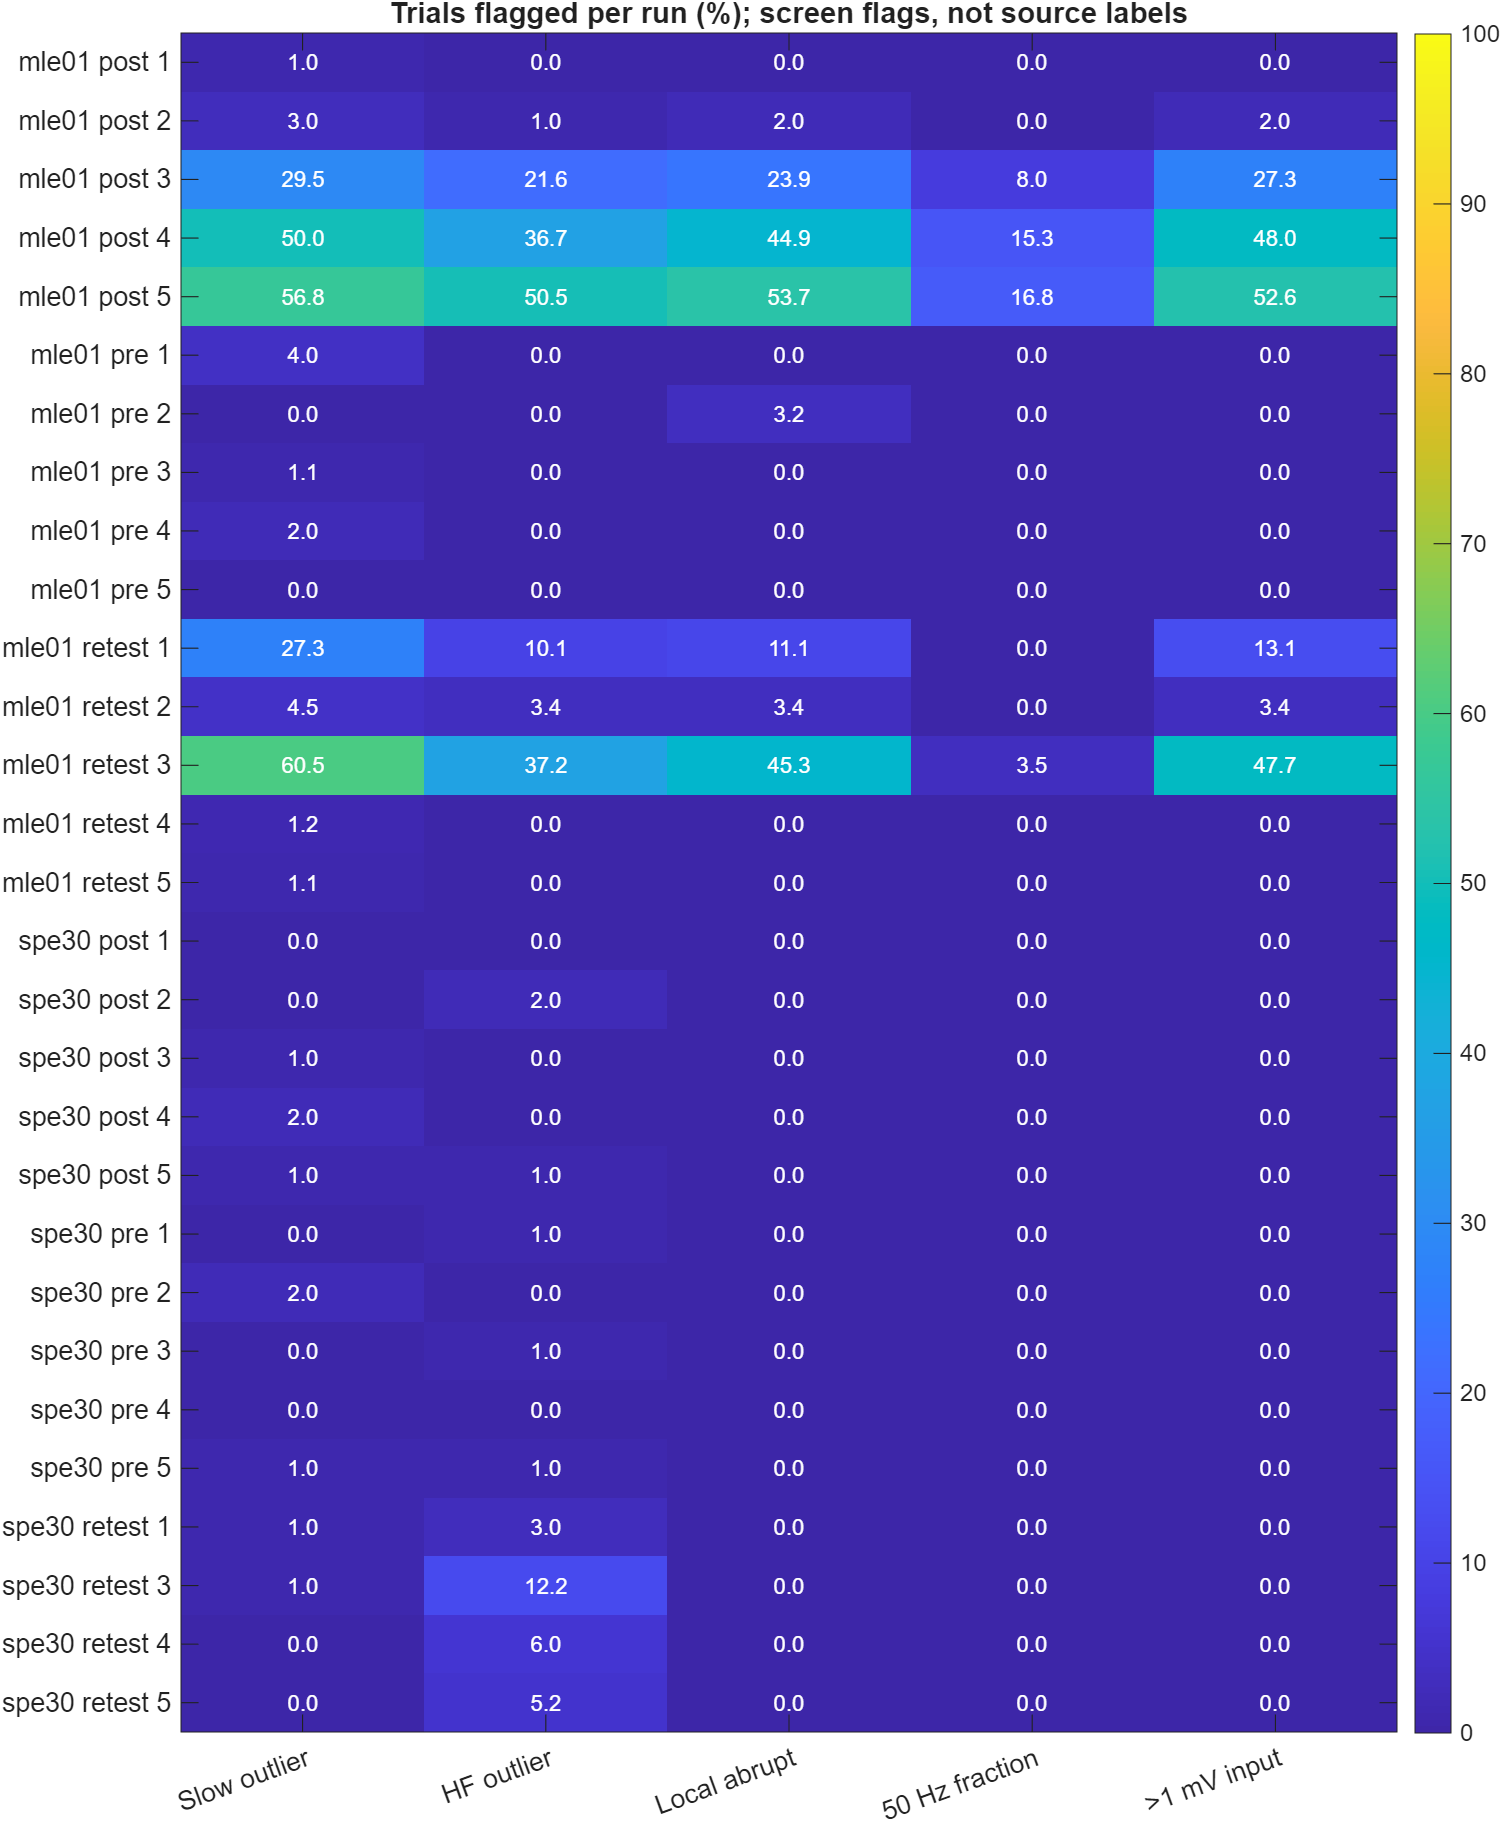
\includegraphics[width=.9\linewidth,height=.69\textheight,keepaspectratio]{figures/run_screen_rates.png}
\caption{Input-screen results for all eligible trials in the 29 pilot recordings. Colours and printed values show the percentage of trials flagged per recording; these are screen flags, not confirmed artifact-source labels. ``50 Hz fraction'' denotes the line-frequency screen.}\label{fig:heatmap}
\end{figure}
\clearpage
\section{Interpretation}
The pilot establishes that some inputs require quality handling, especially the large mle01 disturbances. It does not establish that reconstructive cleaning is necessary rather than rejection, nor that FORCe can reliably repair these examples. Higher-frequency spe30 features and slower deflections need review before source labels or prevalence claims are assigned. Without EOG/EMG, spectral and morphological evidence remains suggestive \cite{whitham,plochl}.

Target-onset markers (code 300) occur between 0.872 and 0.006 s before movement, with median 0.278 s before movement. Movement locking therefore mixes different target-relative timings. Target- and movement-aligned averages are included as context in Section~\ref{sec:eventcontext}. Neither identifies a visual component on its own. The input averages also do not establish a displaced-minus-non-displaced ERP component or its preservation by cleaning \cite{graz}.

\section{Inputs for expert review}\label{sec:review}
\subsection*{Informal expert review}
A brief review of the representative traces would help establish whether the suspected features warrant cleaning for the ErrP analysis. Comments on clear or uncertain examples are welcome; completing an assessment for every plot is not required.
\begin{itemize}
\item Do the slower deflections and higher-frequency activity look like artifacts, physiological activity, or remain uncertain?
\item Which examples, channels and time intervals are affected, and what source seems plausible?
\item Do these features warrant cleaning or trial rejection for our analysis, particularly within 0.4--0.8 s?
\end{itemize}
\noindent\textbf{Optional comments (please refer to review numbers):}\par
\vspace{0.4cm}\noindent\rule{\linewidth}{0.4pt}\par
\vspace{0.4cm}\noindent\rule{\linewidth}{0.4pt}\par
\vspace{0.4cm}\noindent\rule{\linewidth}{0.4pt}\par
This is an informal expert assessment to guide the next comparison, not systematic artifact annotation or a validation of artifact prevalence.

Figures show all eight channels. Channel medians are removed and traces vertically separated only for display; the spacing is printed in microvolts. Black dotted lines mark movement, brown/orange dashed lines target and green dashed lines displacement when recorded. Spectra show PSD estimates averaged across three separate one-second windows. Labels 1 and 2 denote non-displaced and displaced trials respectively. No figure displays a FORCe output.

\clearpage
\subsection*{Review 1: mle01 / post / run 1 / trial 64}
\textbf{Randomly selected example:} one eligible trial sampled uniformly from this recording; not certified clean.
\begin{center}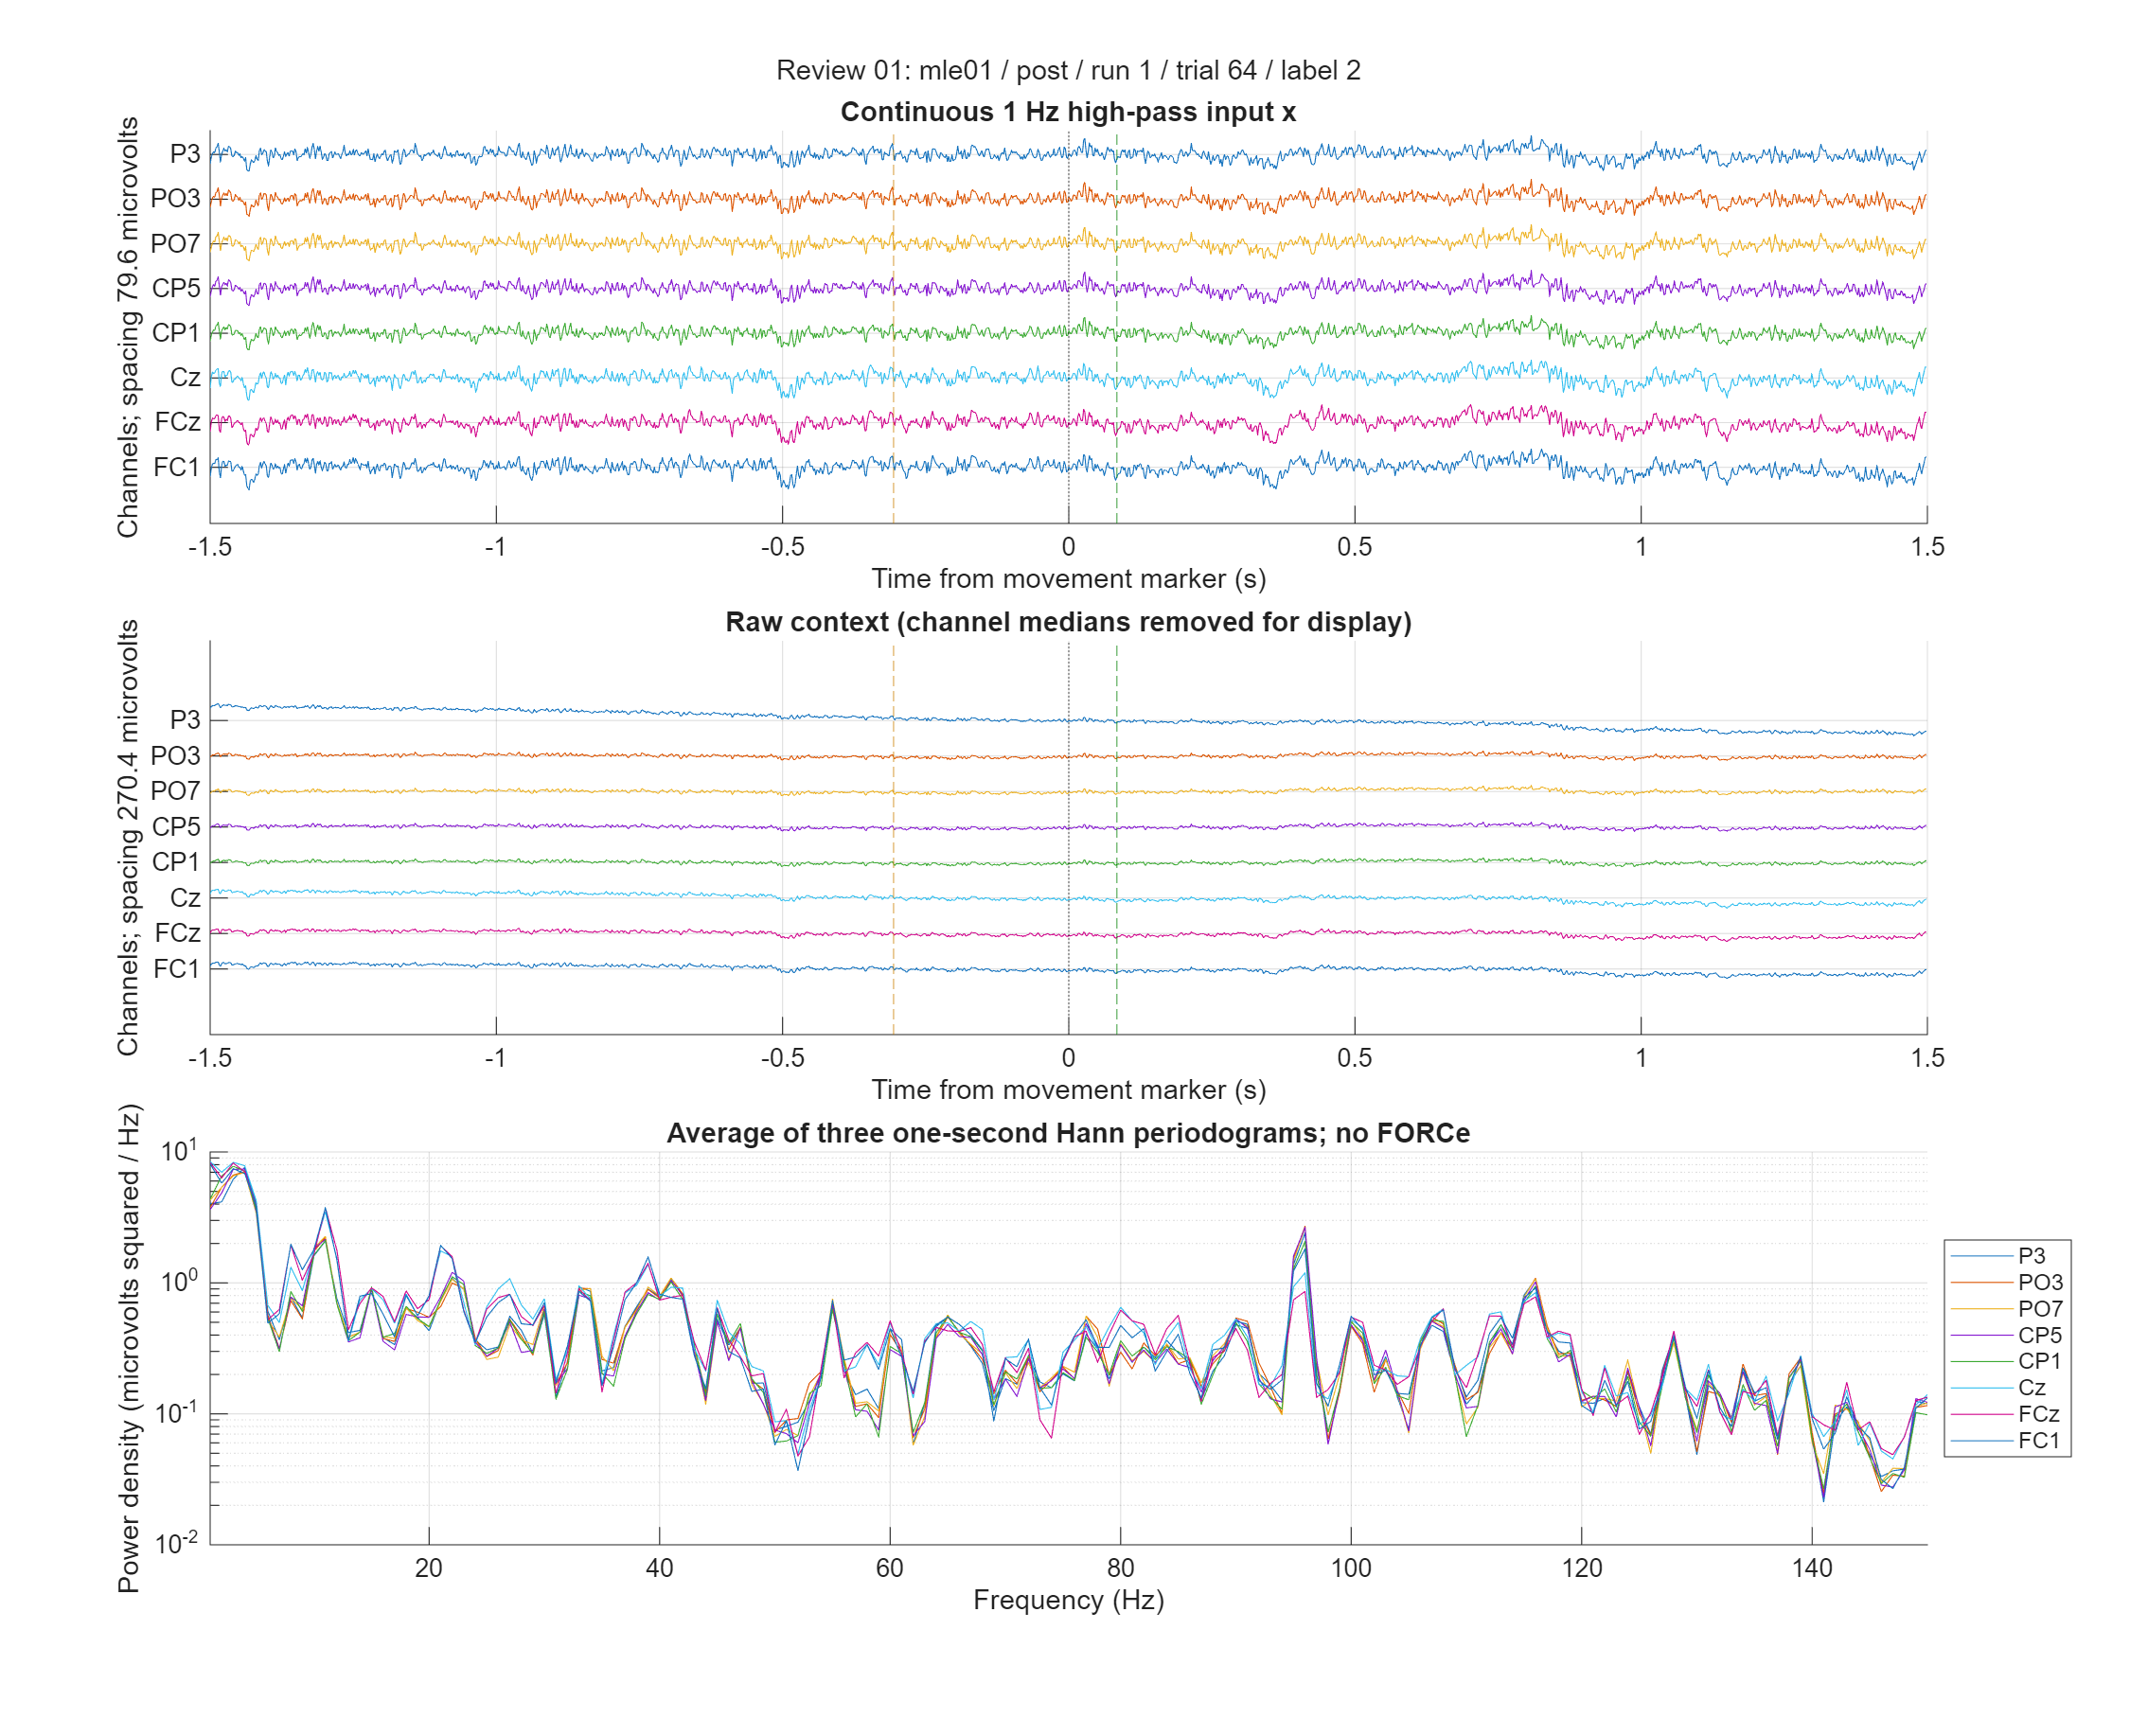
\includegraphics[width=\linewidth,height=.78\textheight,keepaspectratio]{figures/review_001.png}\end{center}\clearpage
\subsection*{Review 20: spe30 / post / run 5 / trial 61}
\textbf{Randomly selected example:} one eligible trial sampled uniformly from this recording; not certified clean.
\begin{center}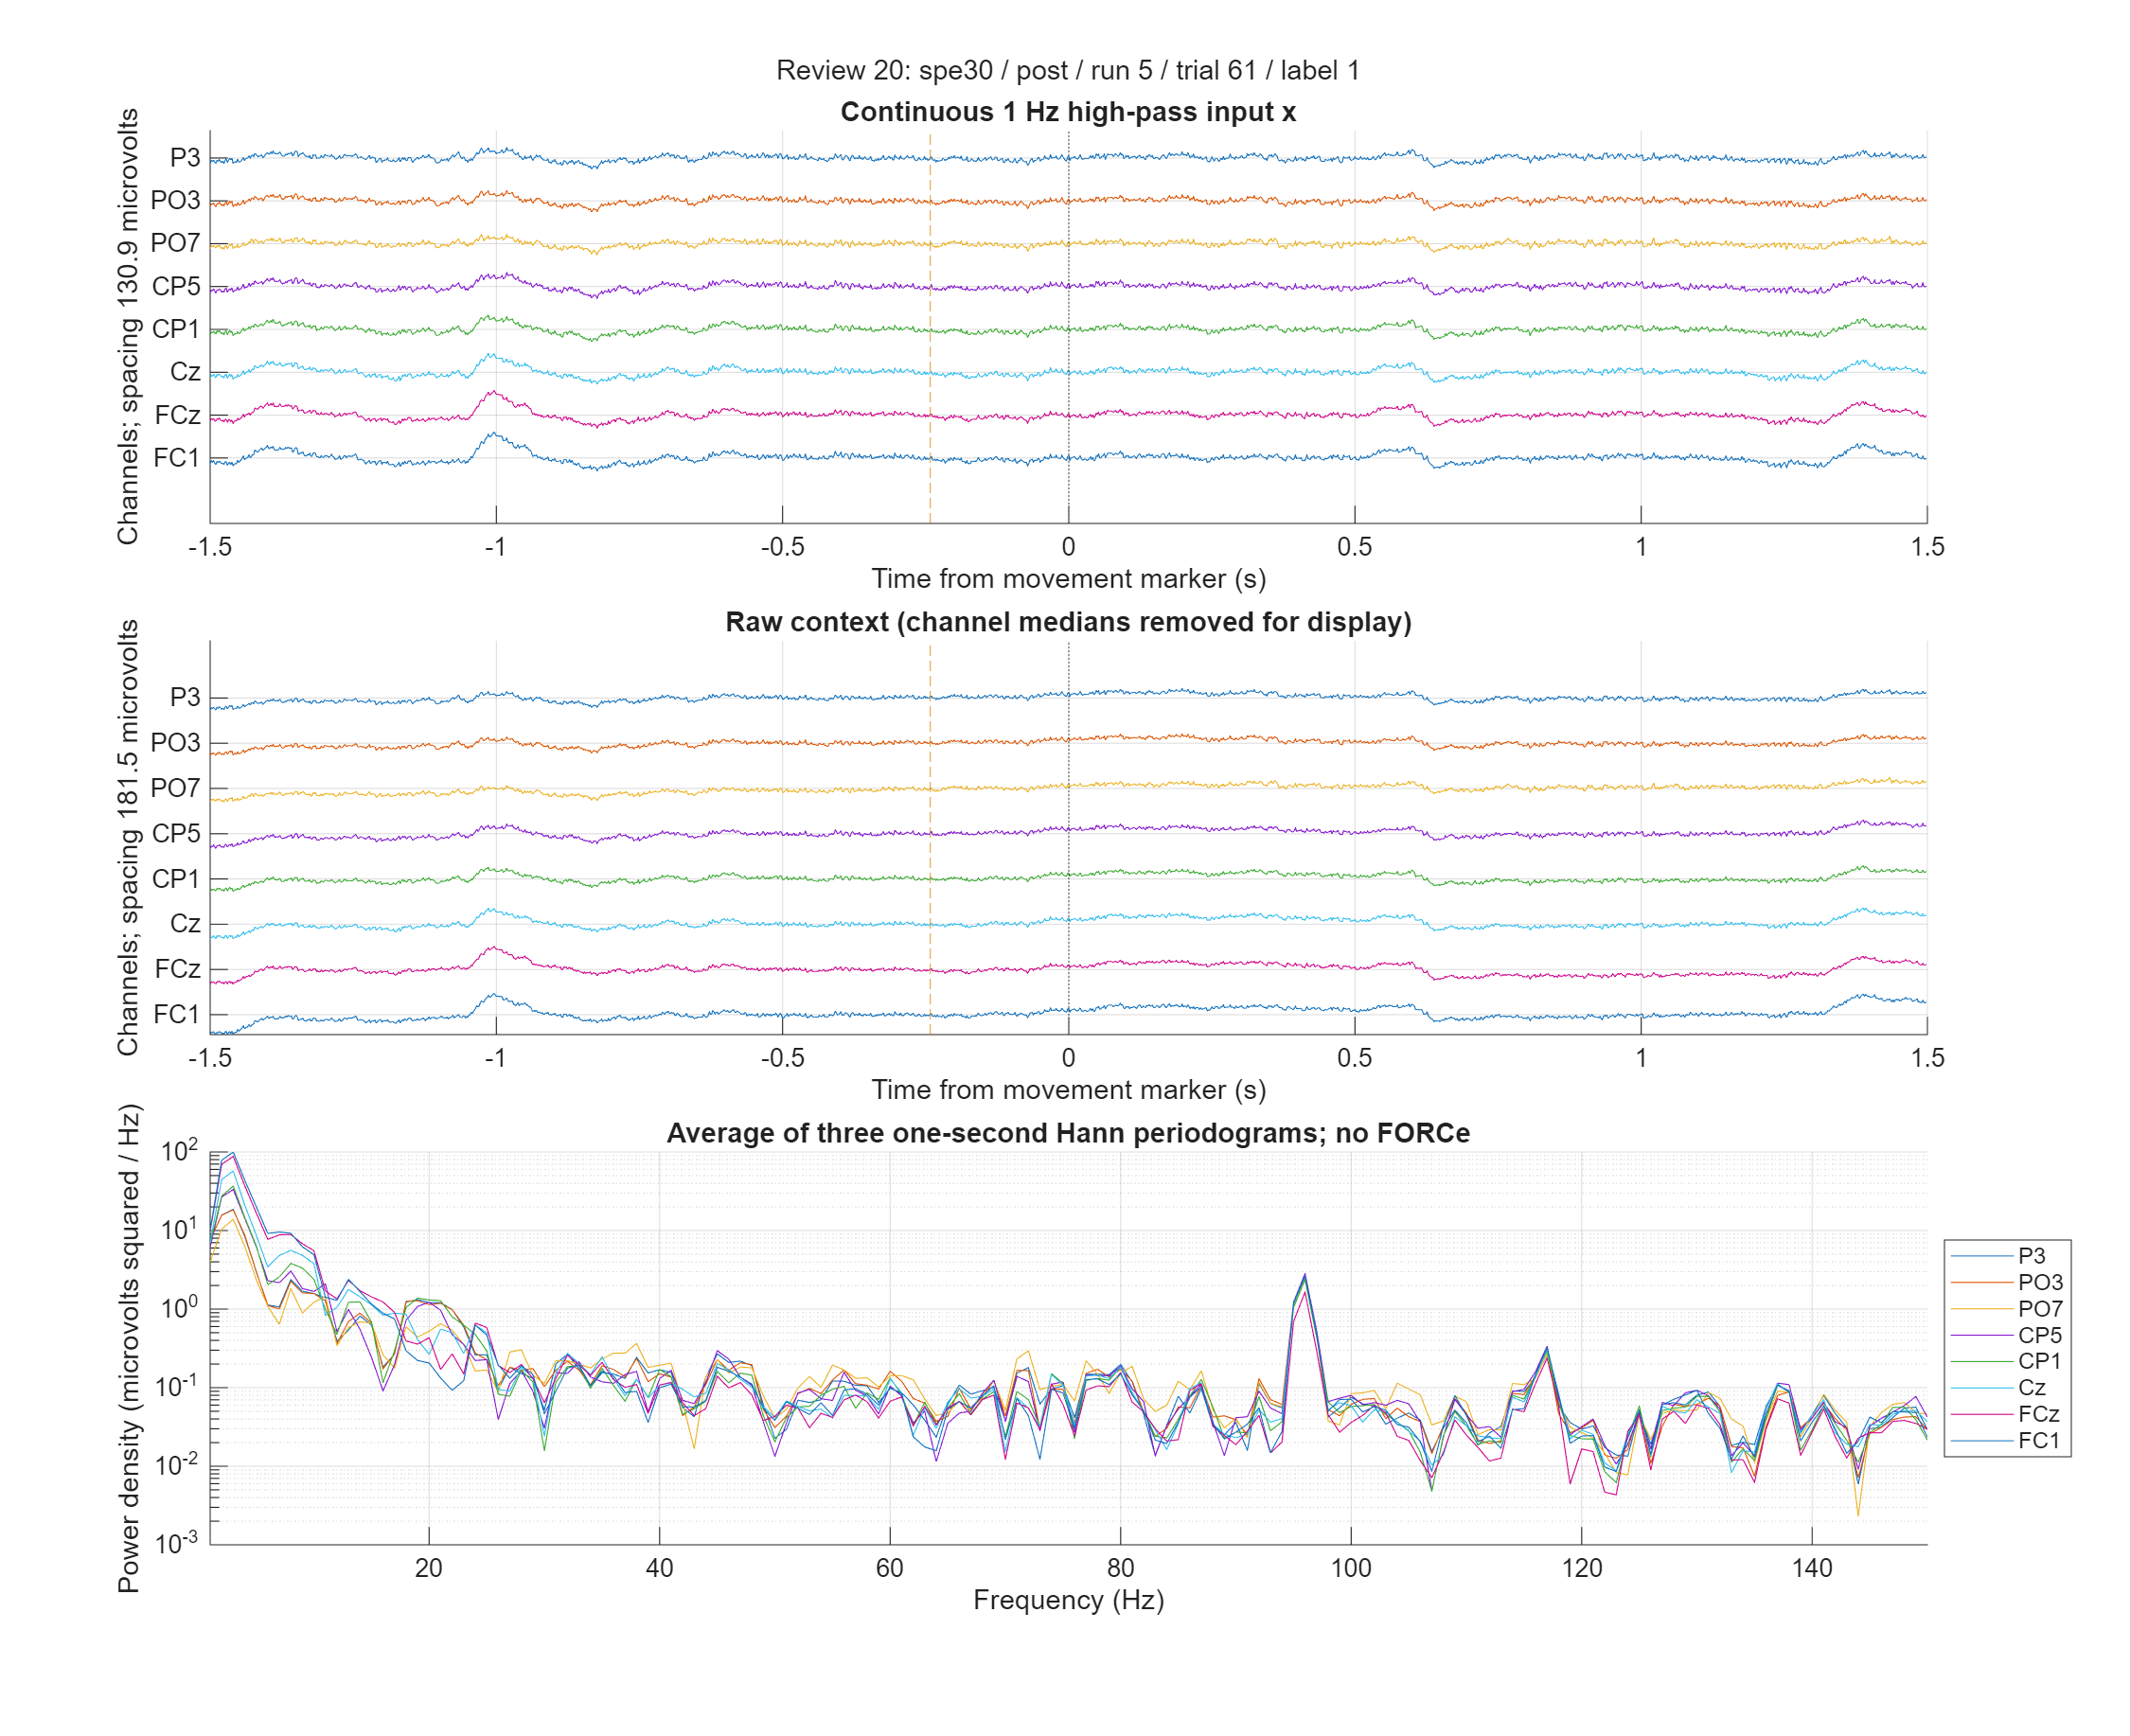
\includegraphics[width=\linewidth,height=.78\textheight,keepaspectratio]{figures/review_020.png}\end{center}\clearpage
\subsection*{Review 30: mle01 / post / run 3 / trial 72}
\textbf{Selected for suspected contamination: gross excursion.} Large P3 disturbances are inconsistent with an ordinary EEG interpretation. The large display spacing compresses other channels.
\begin{center}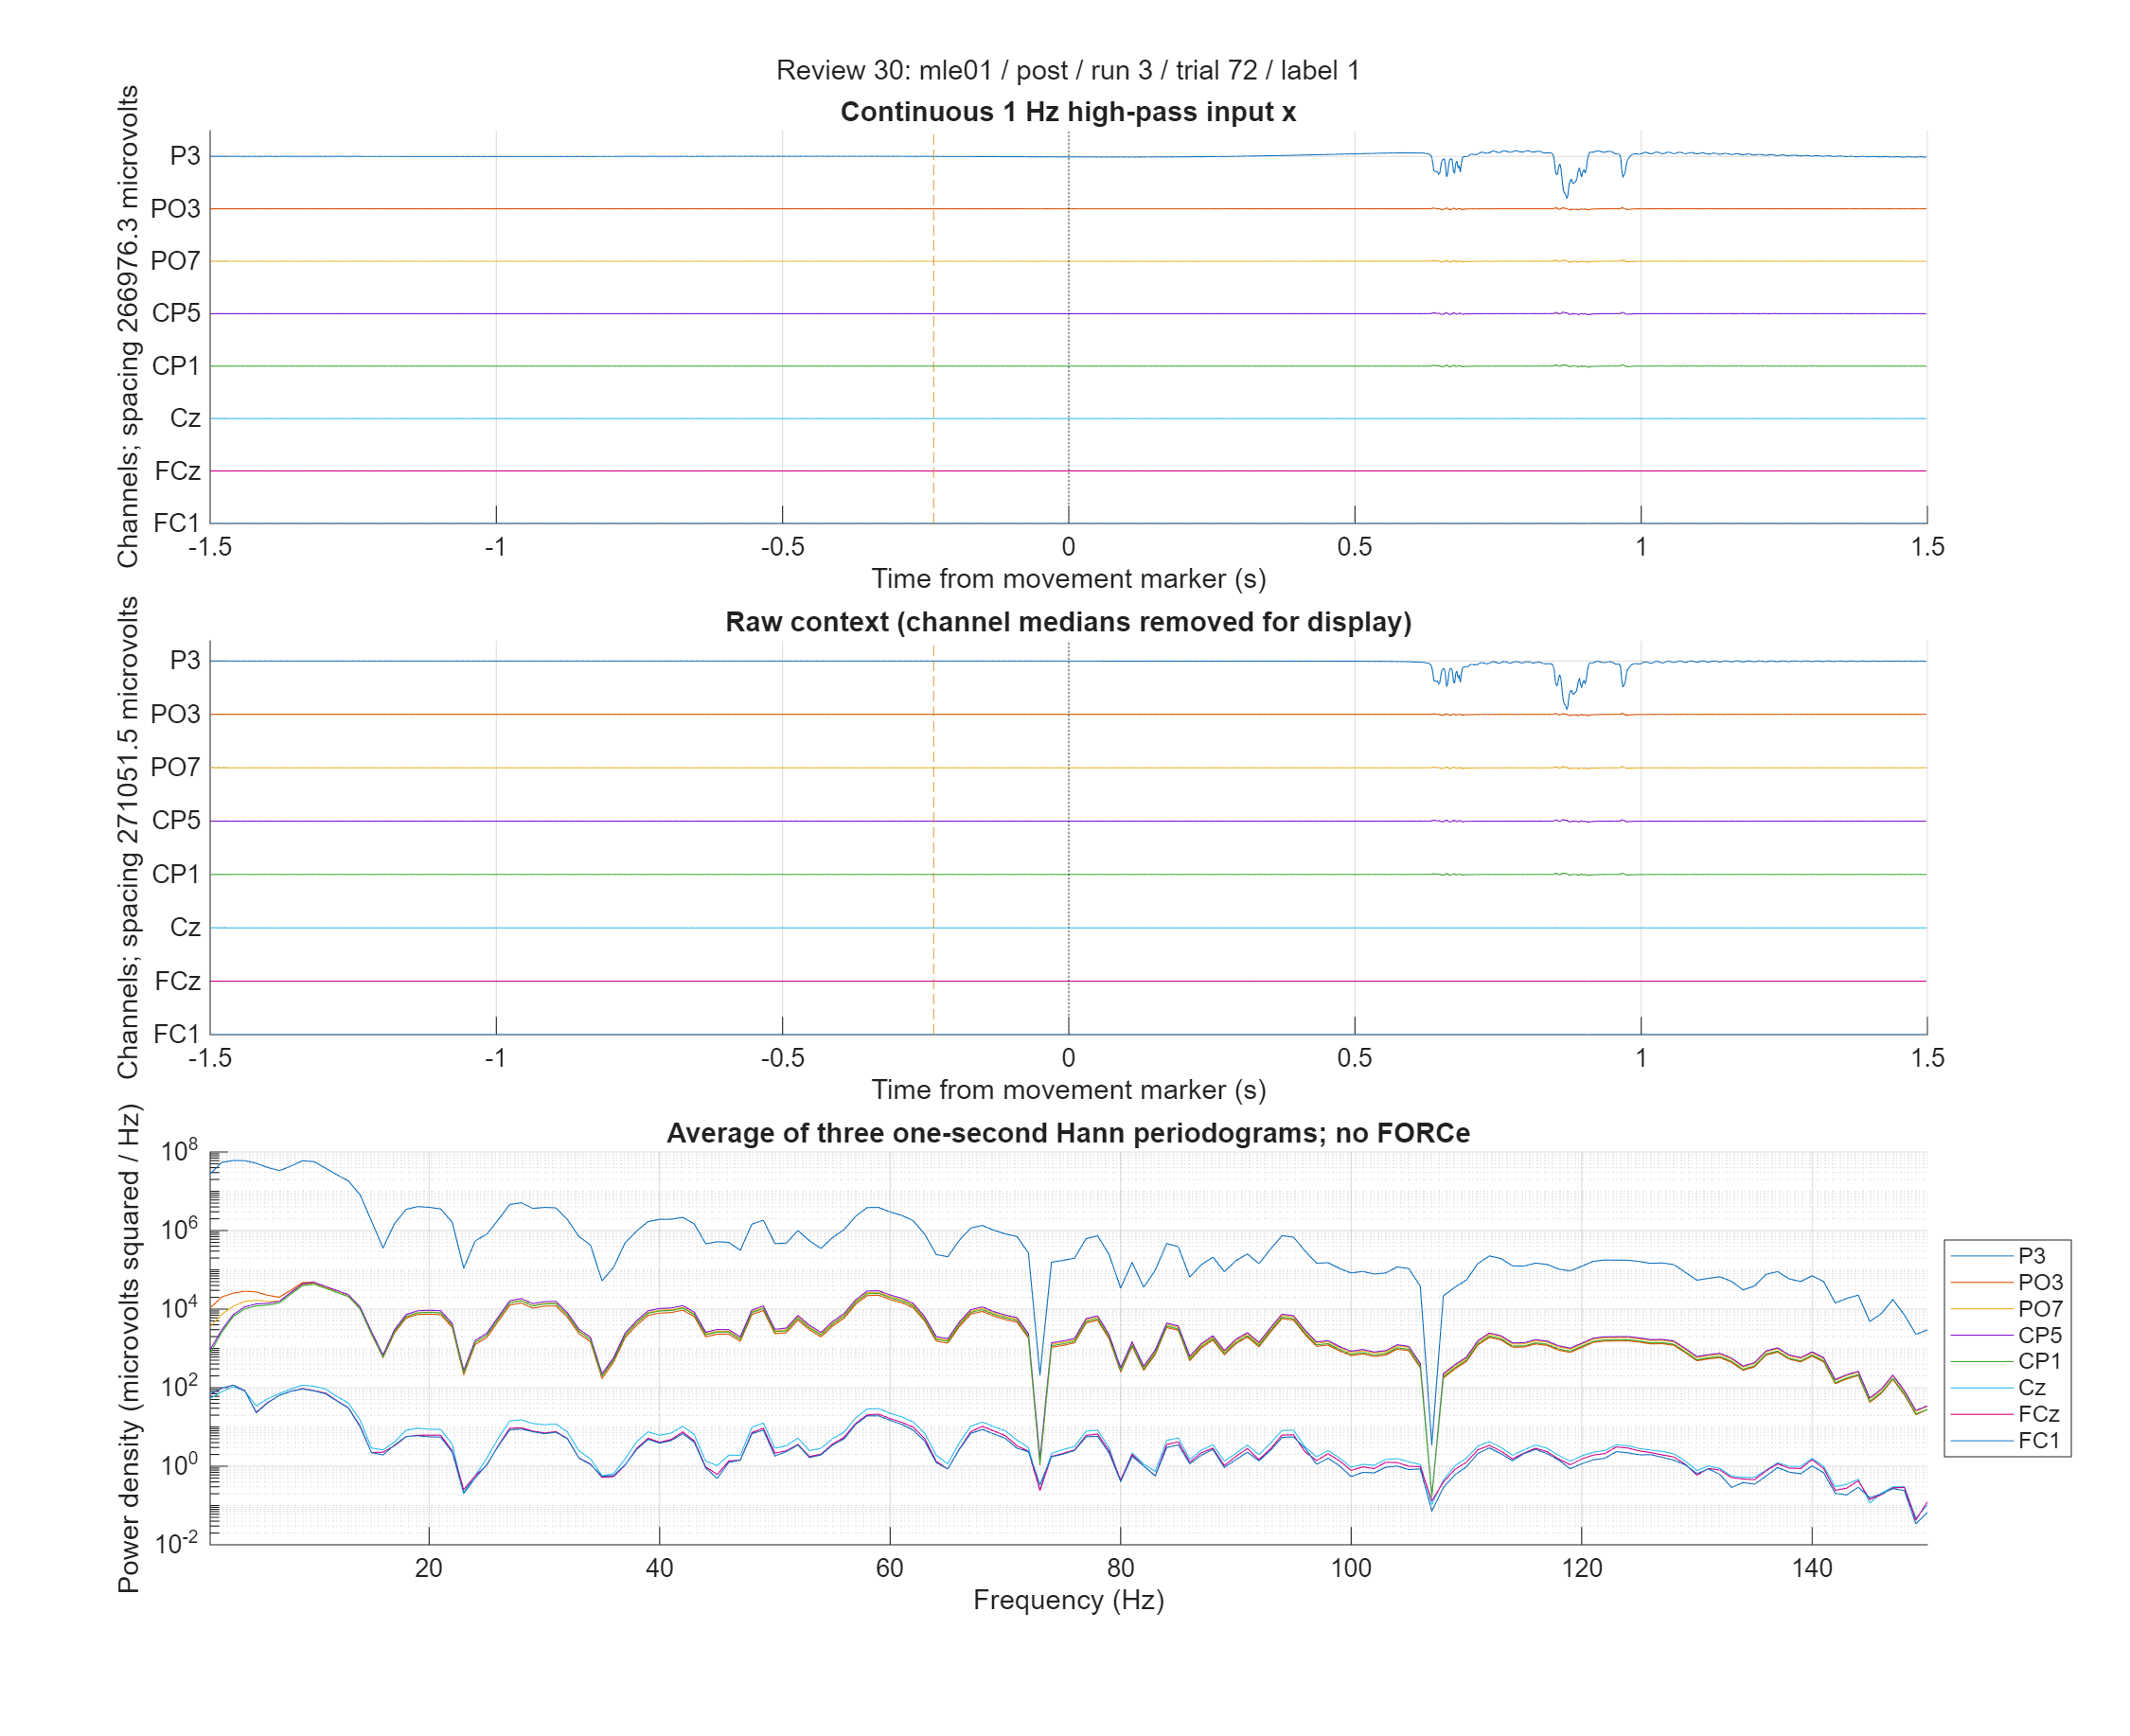
\includegraphics[width=\linewidth,height=.78\textheight,keepaspectratio]{figures/review_030.png}\end{center}\clearpage
\subsection*{Review 31: mle01 / pre / run 2 / trial 32}
\textbf{Selected for inspection: higher-frequency activity (mle01).} Selected for inspection, but no higher-frequency threshold flag occurs in the bounded mle01 stratum. Source is uncertain.
\begin{center}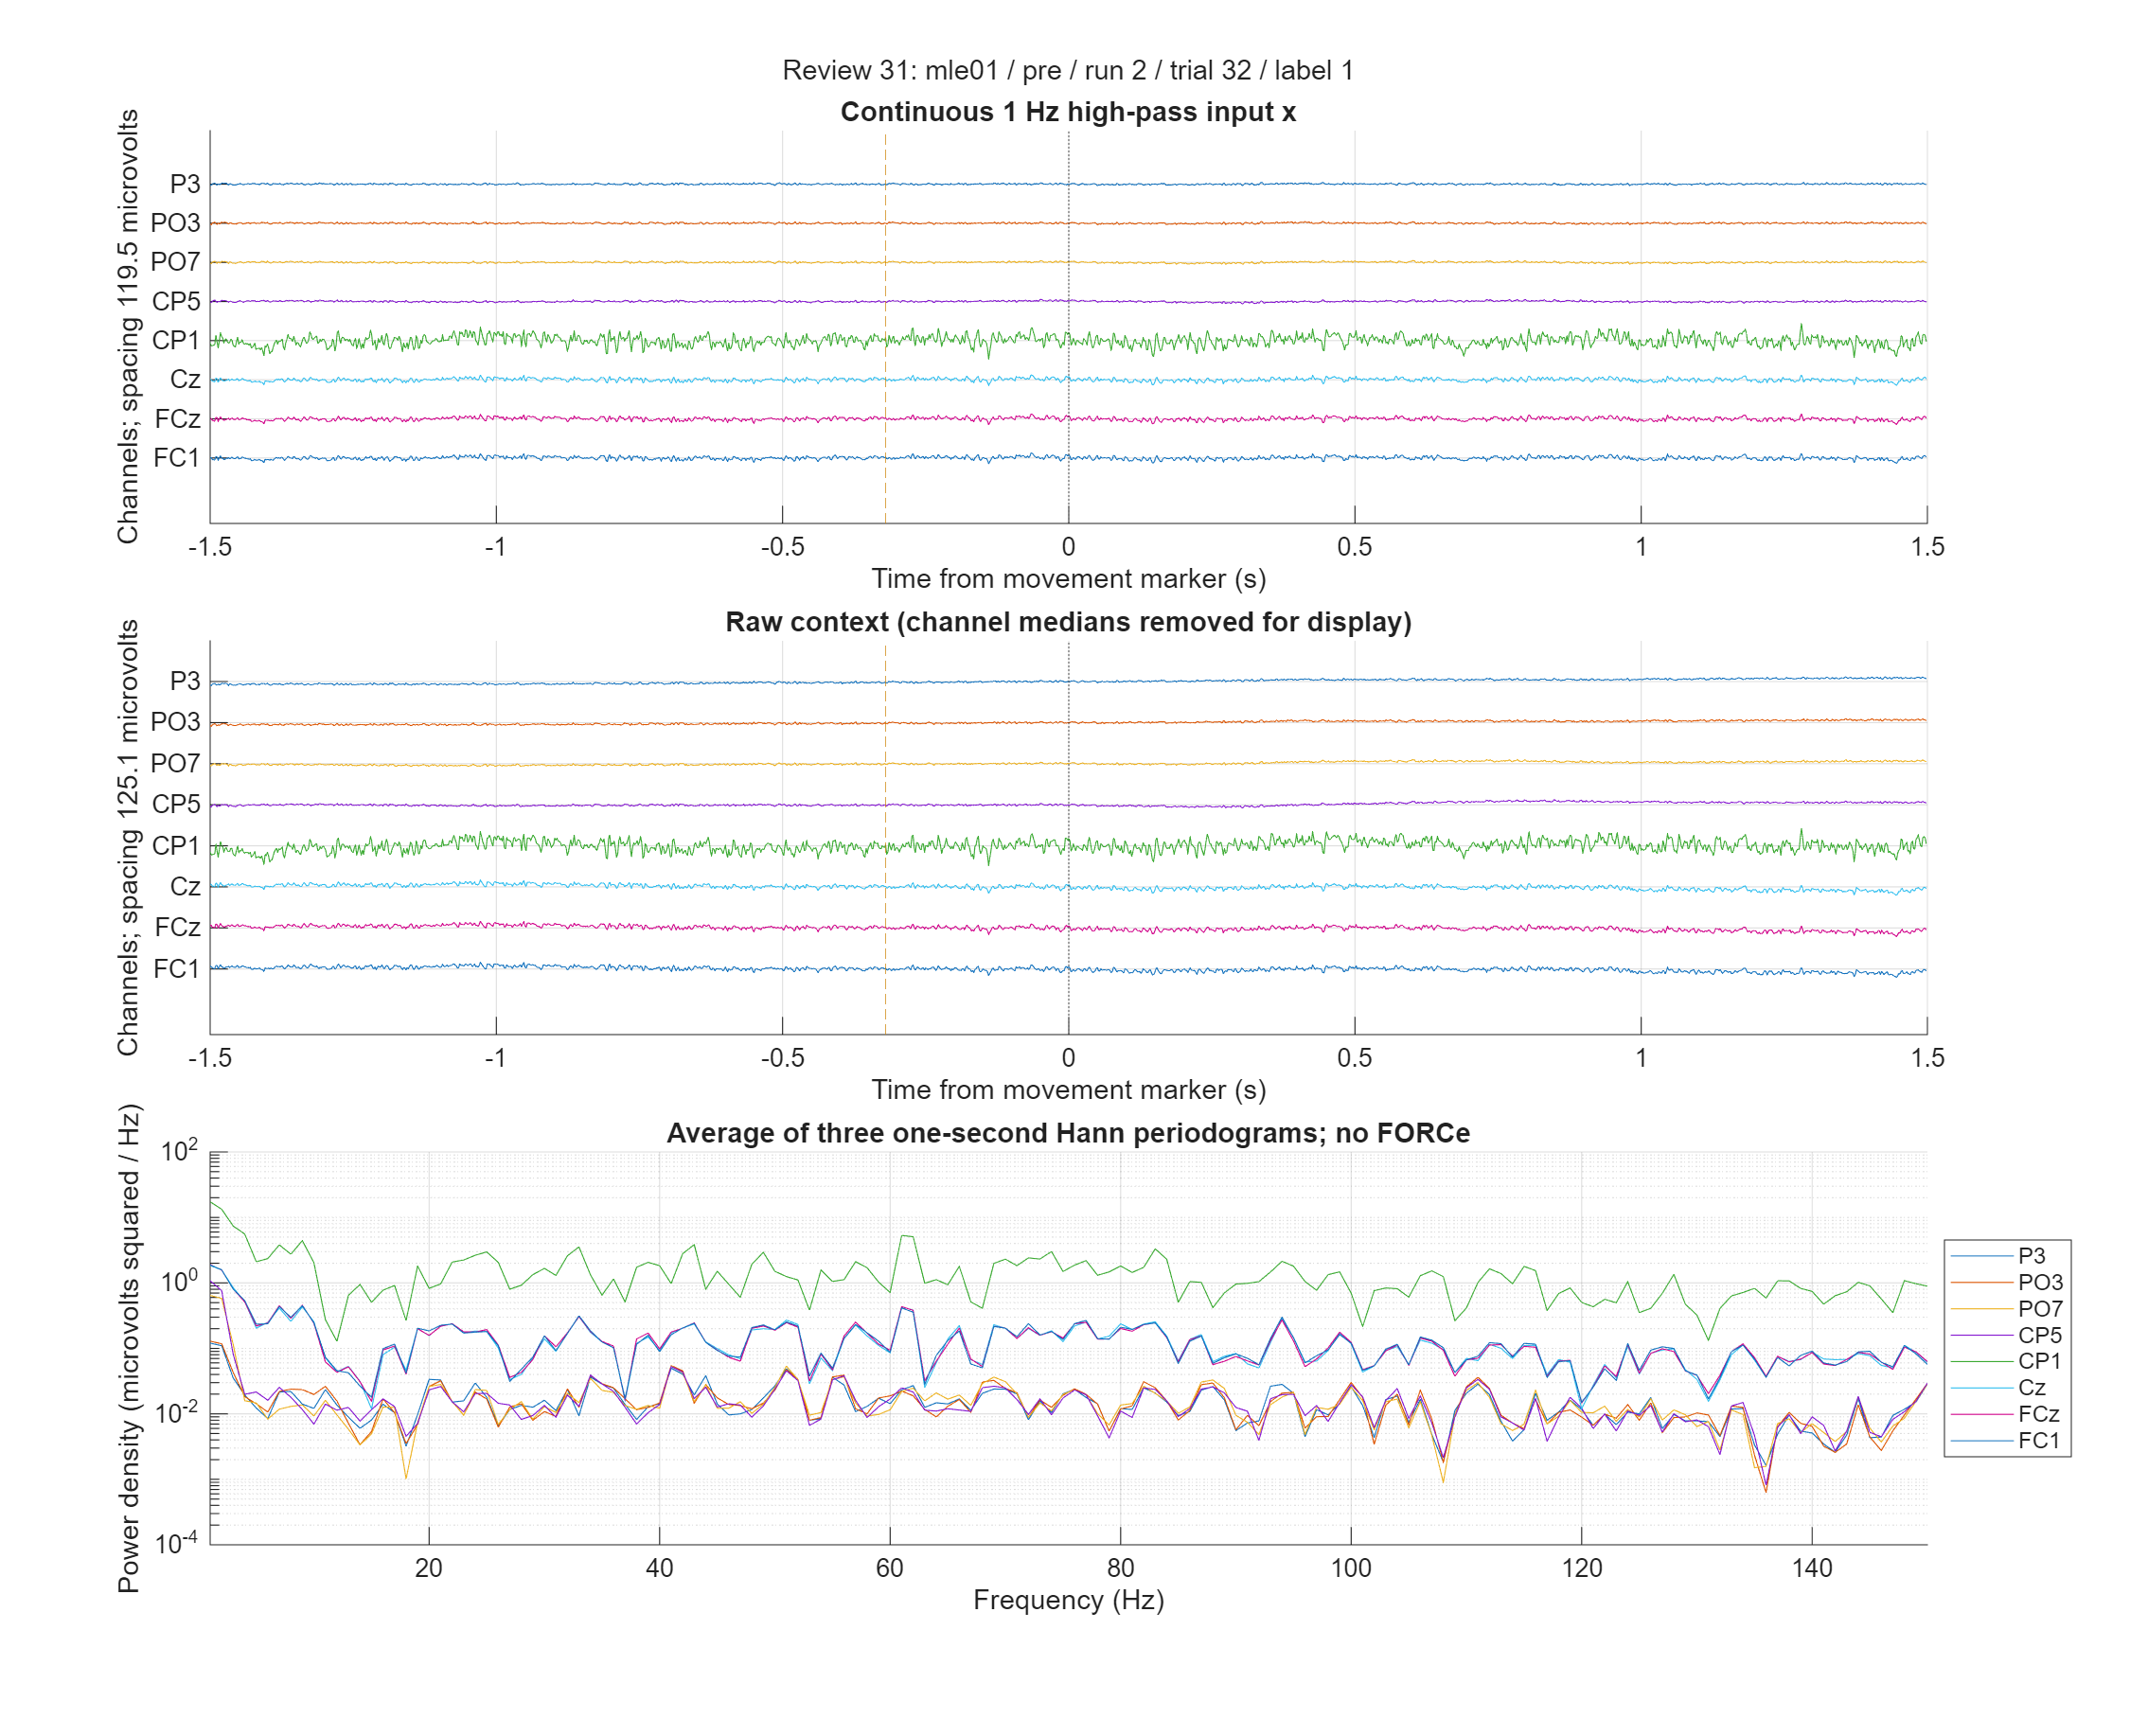
\includegraphics[width=\linewidth,height=.78\textheight,keepaspectratio]{figures/review_031.png}\end{center}\clearpage
\subsection*{Review 32: spe30 / retest / run 4 / trial 50}
\textbf{Selected for suspected contamination: higher-frequency activity (spe30).} Rapid fluctuations are prominent before movement across channels. Muscle, shared noise and neural contributions are not distinguished by this plot.
\begin{center}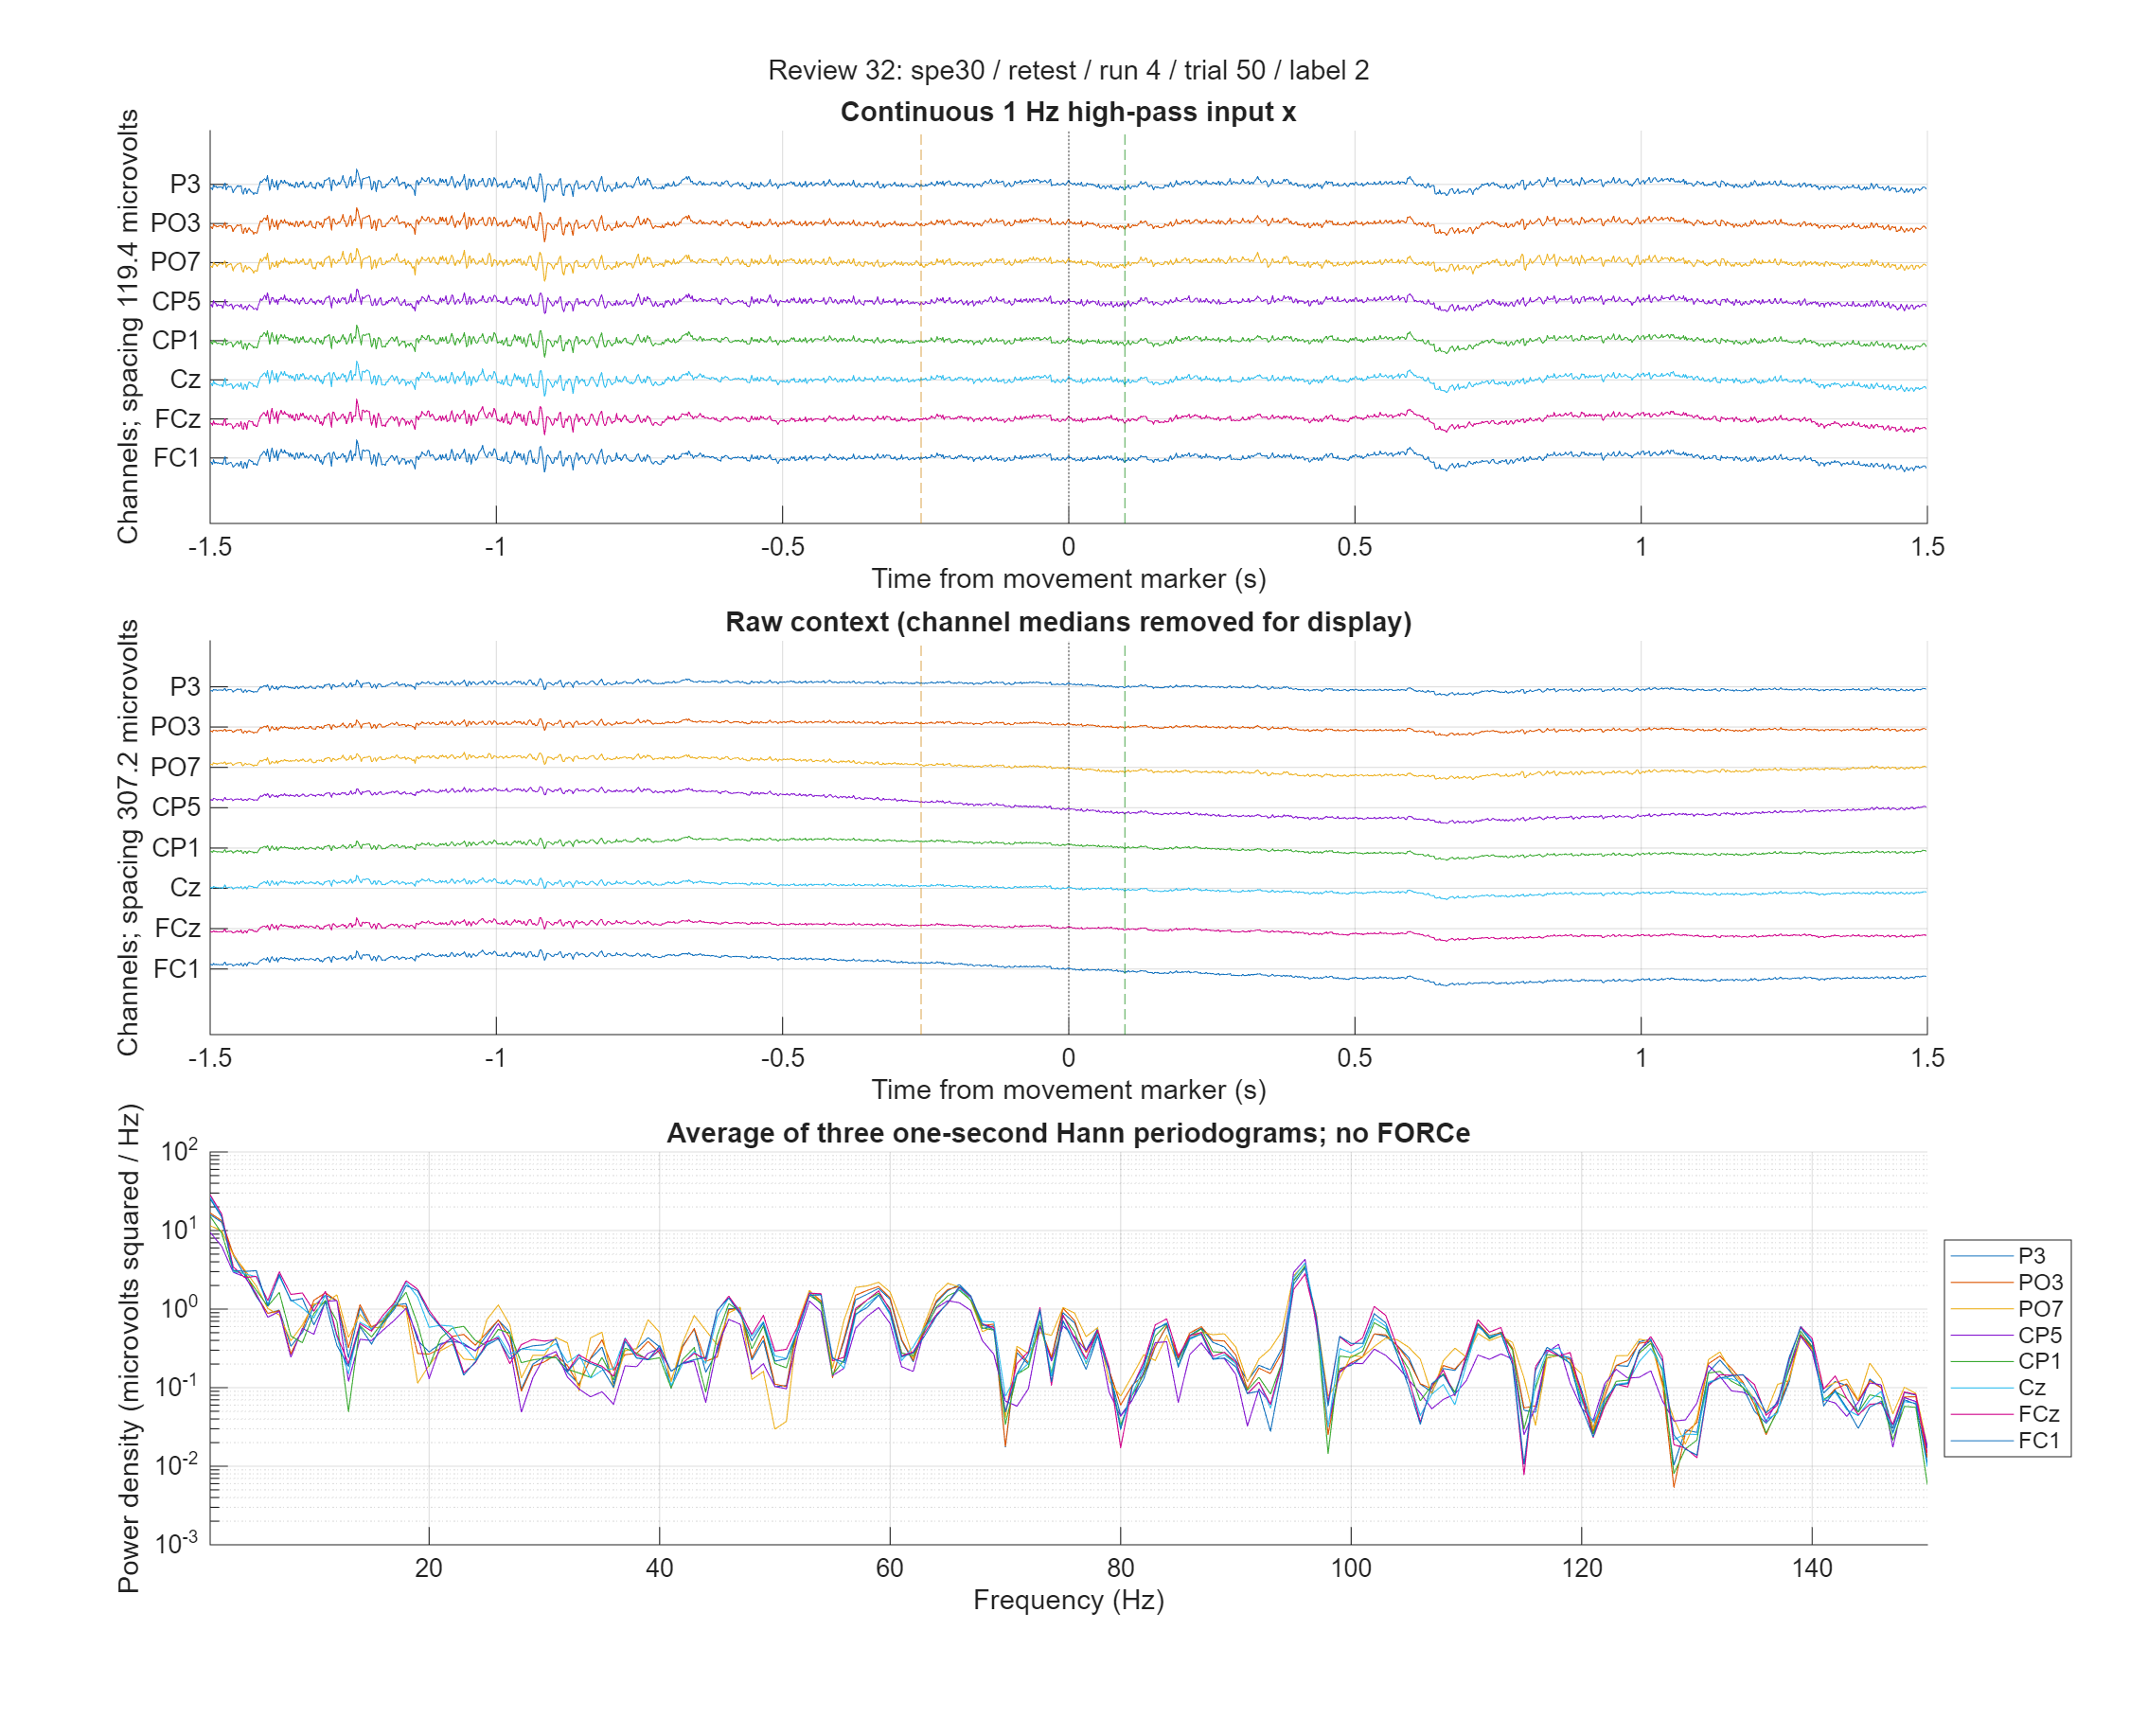
\includegraphics[width=\linewidth,height=.78\textheight,keepaspectratio]{figures/review_032.png}\end{center}\clearpage
\subsection*{Review 33: mle01 / retest / run 1 / trial 10}
\textbf{Selected for suspected contamination: slow deflection (mle01).} Posterior deflections cannot be automatically identified as an ocular artifact.
\begin{center}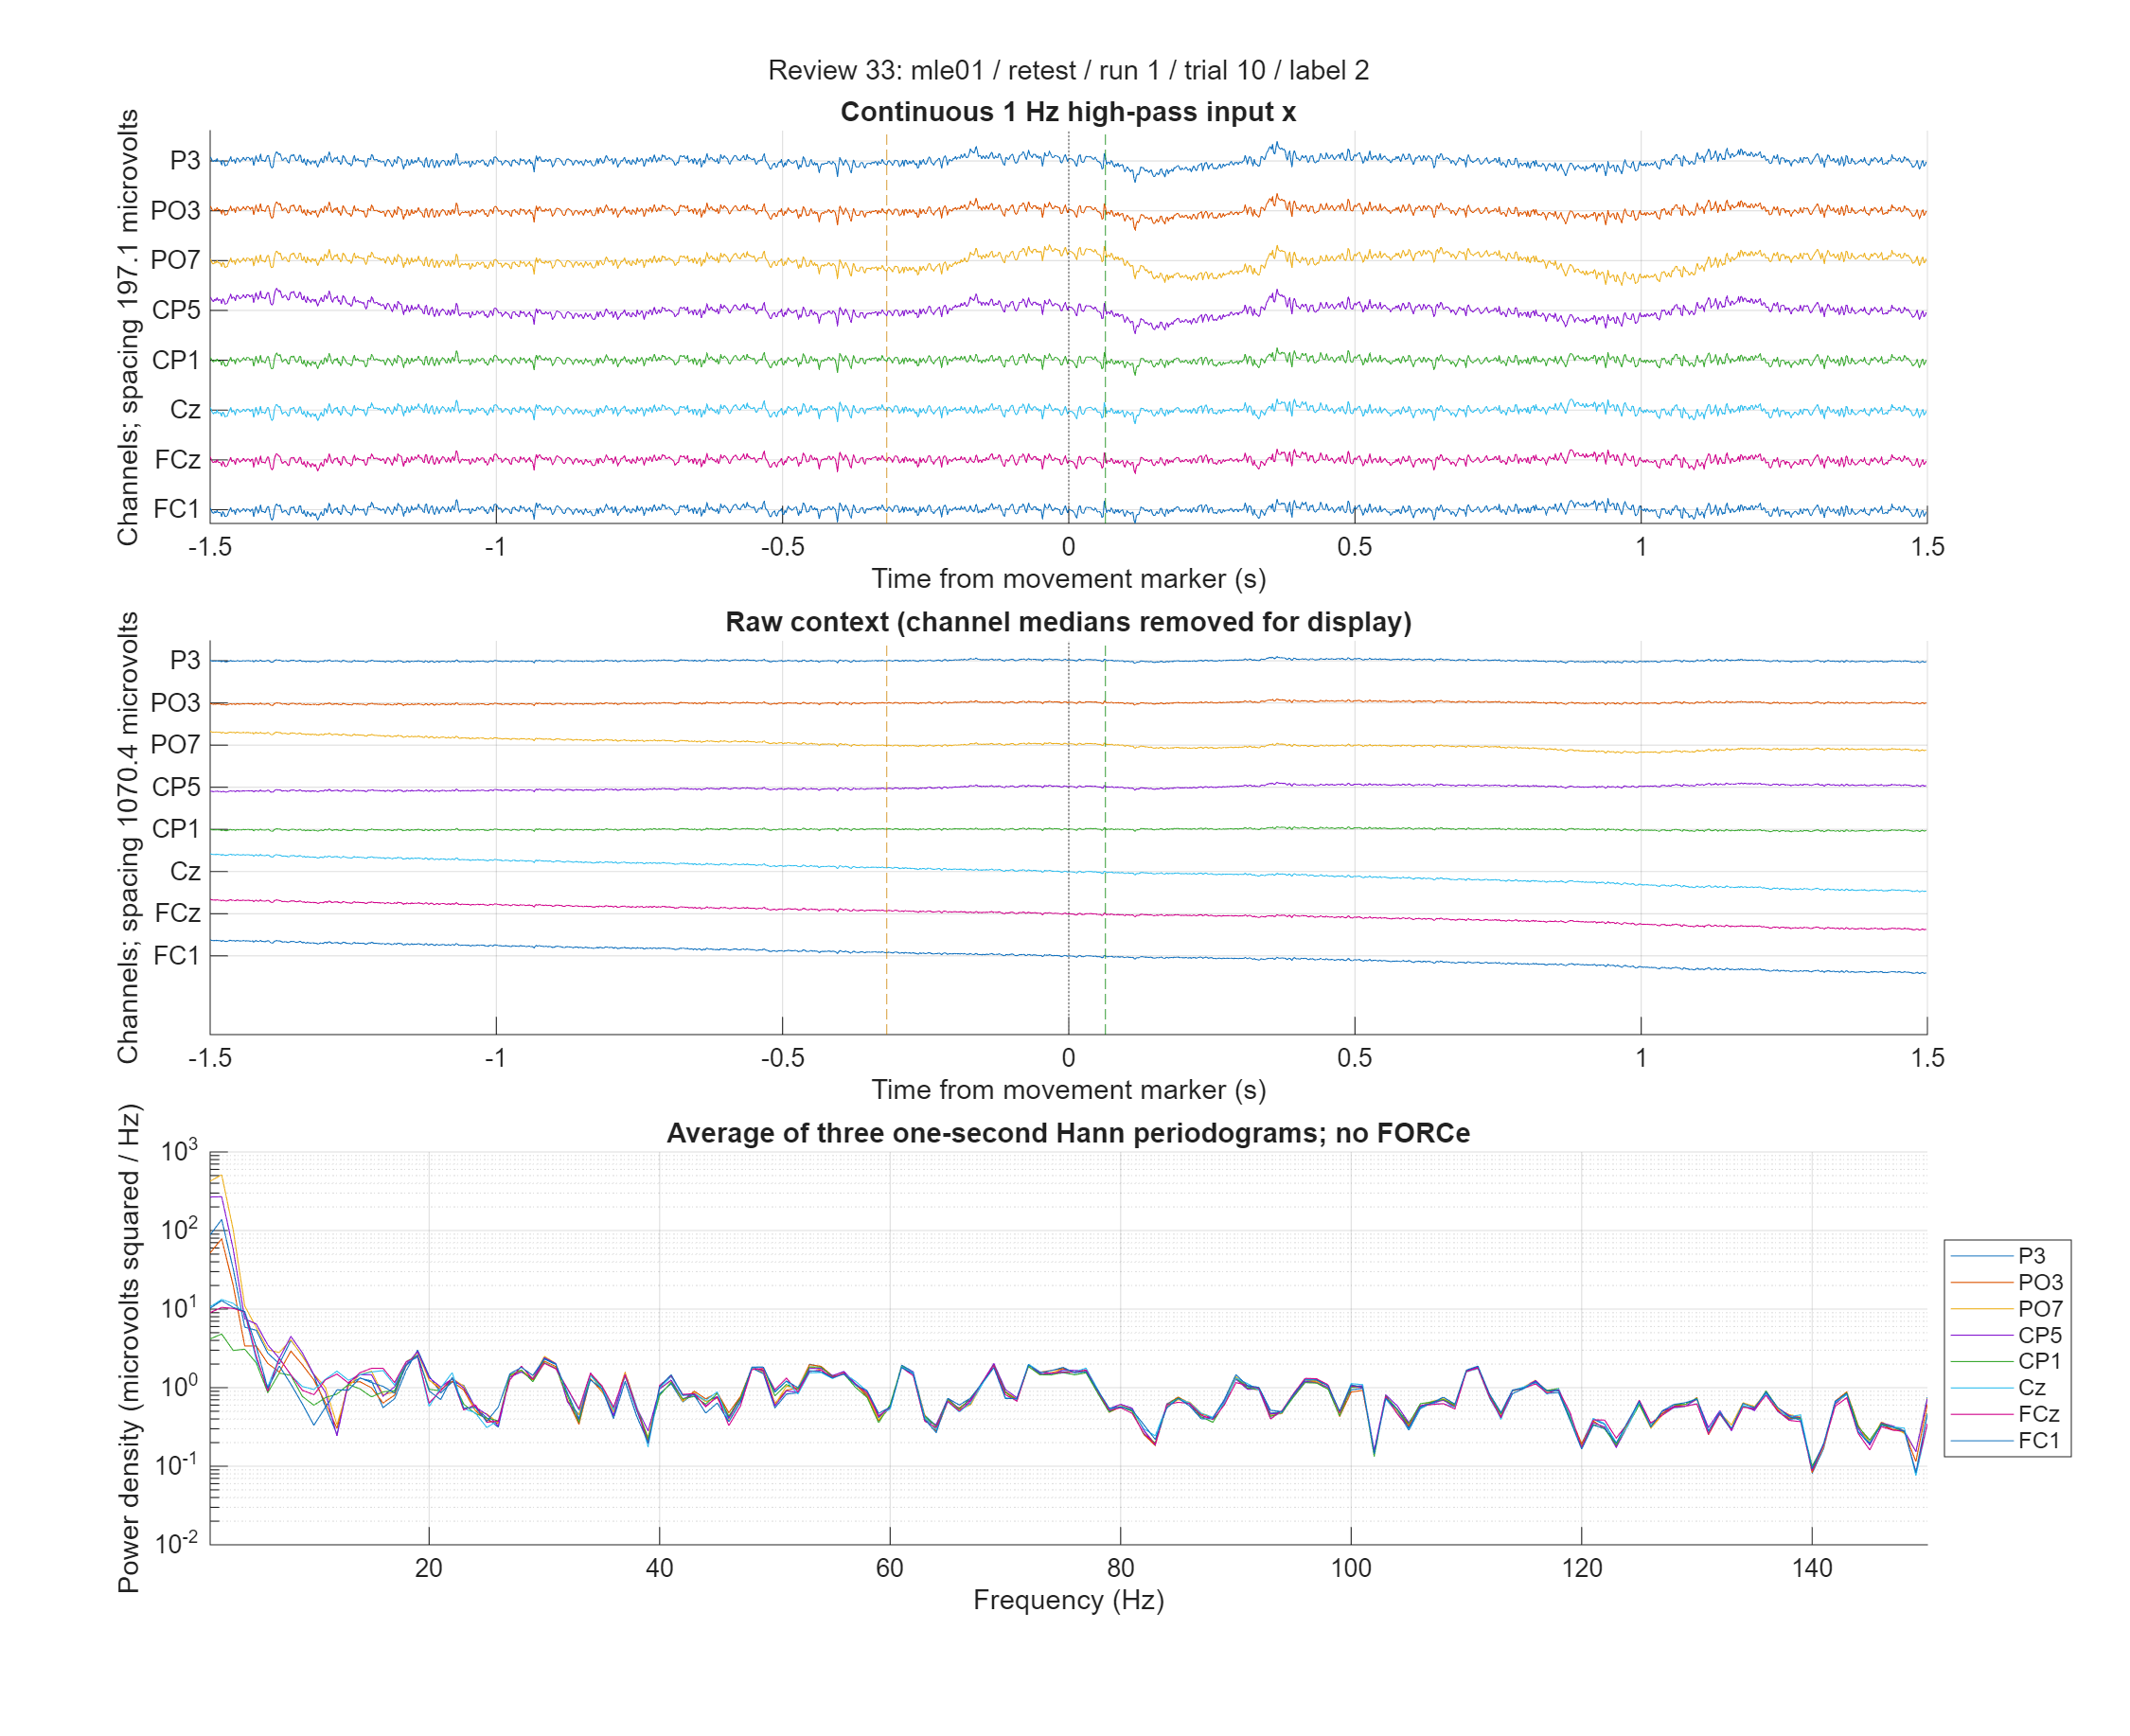
\includegraphics[width=\linewidth,height=.78\textheight,keepaspectratio]{figures/review_033.png}\end{center}\clearpage
\subsection*{Review 34: spe30 / post / run 4 / trial 53}
\textbf{Selected for suspected contamination: slow deflection (spe30).} A broad frontocentral deflection appears late in the interval; source and relevance require review.
\begin{center}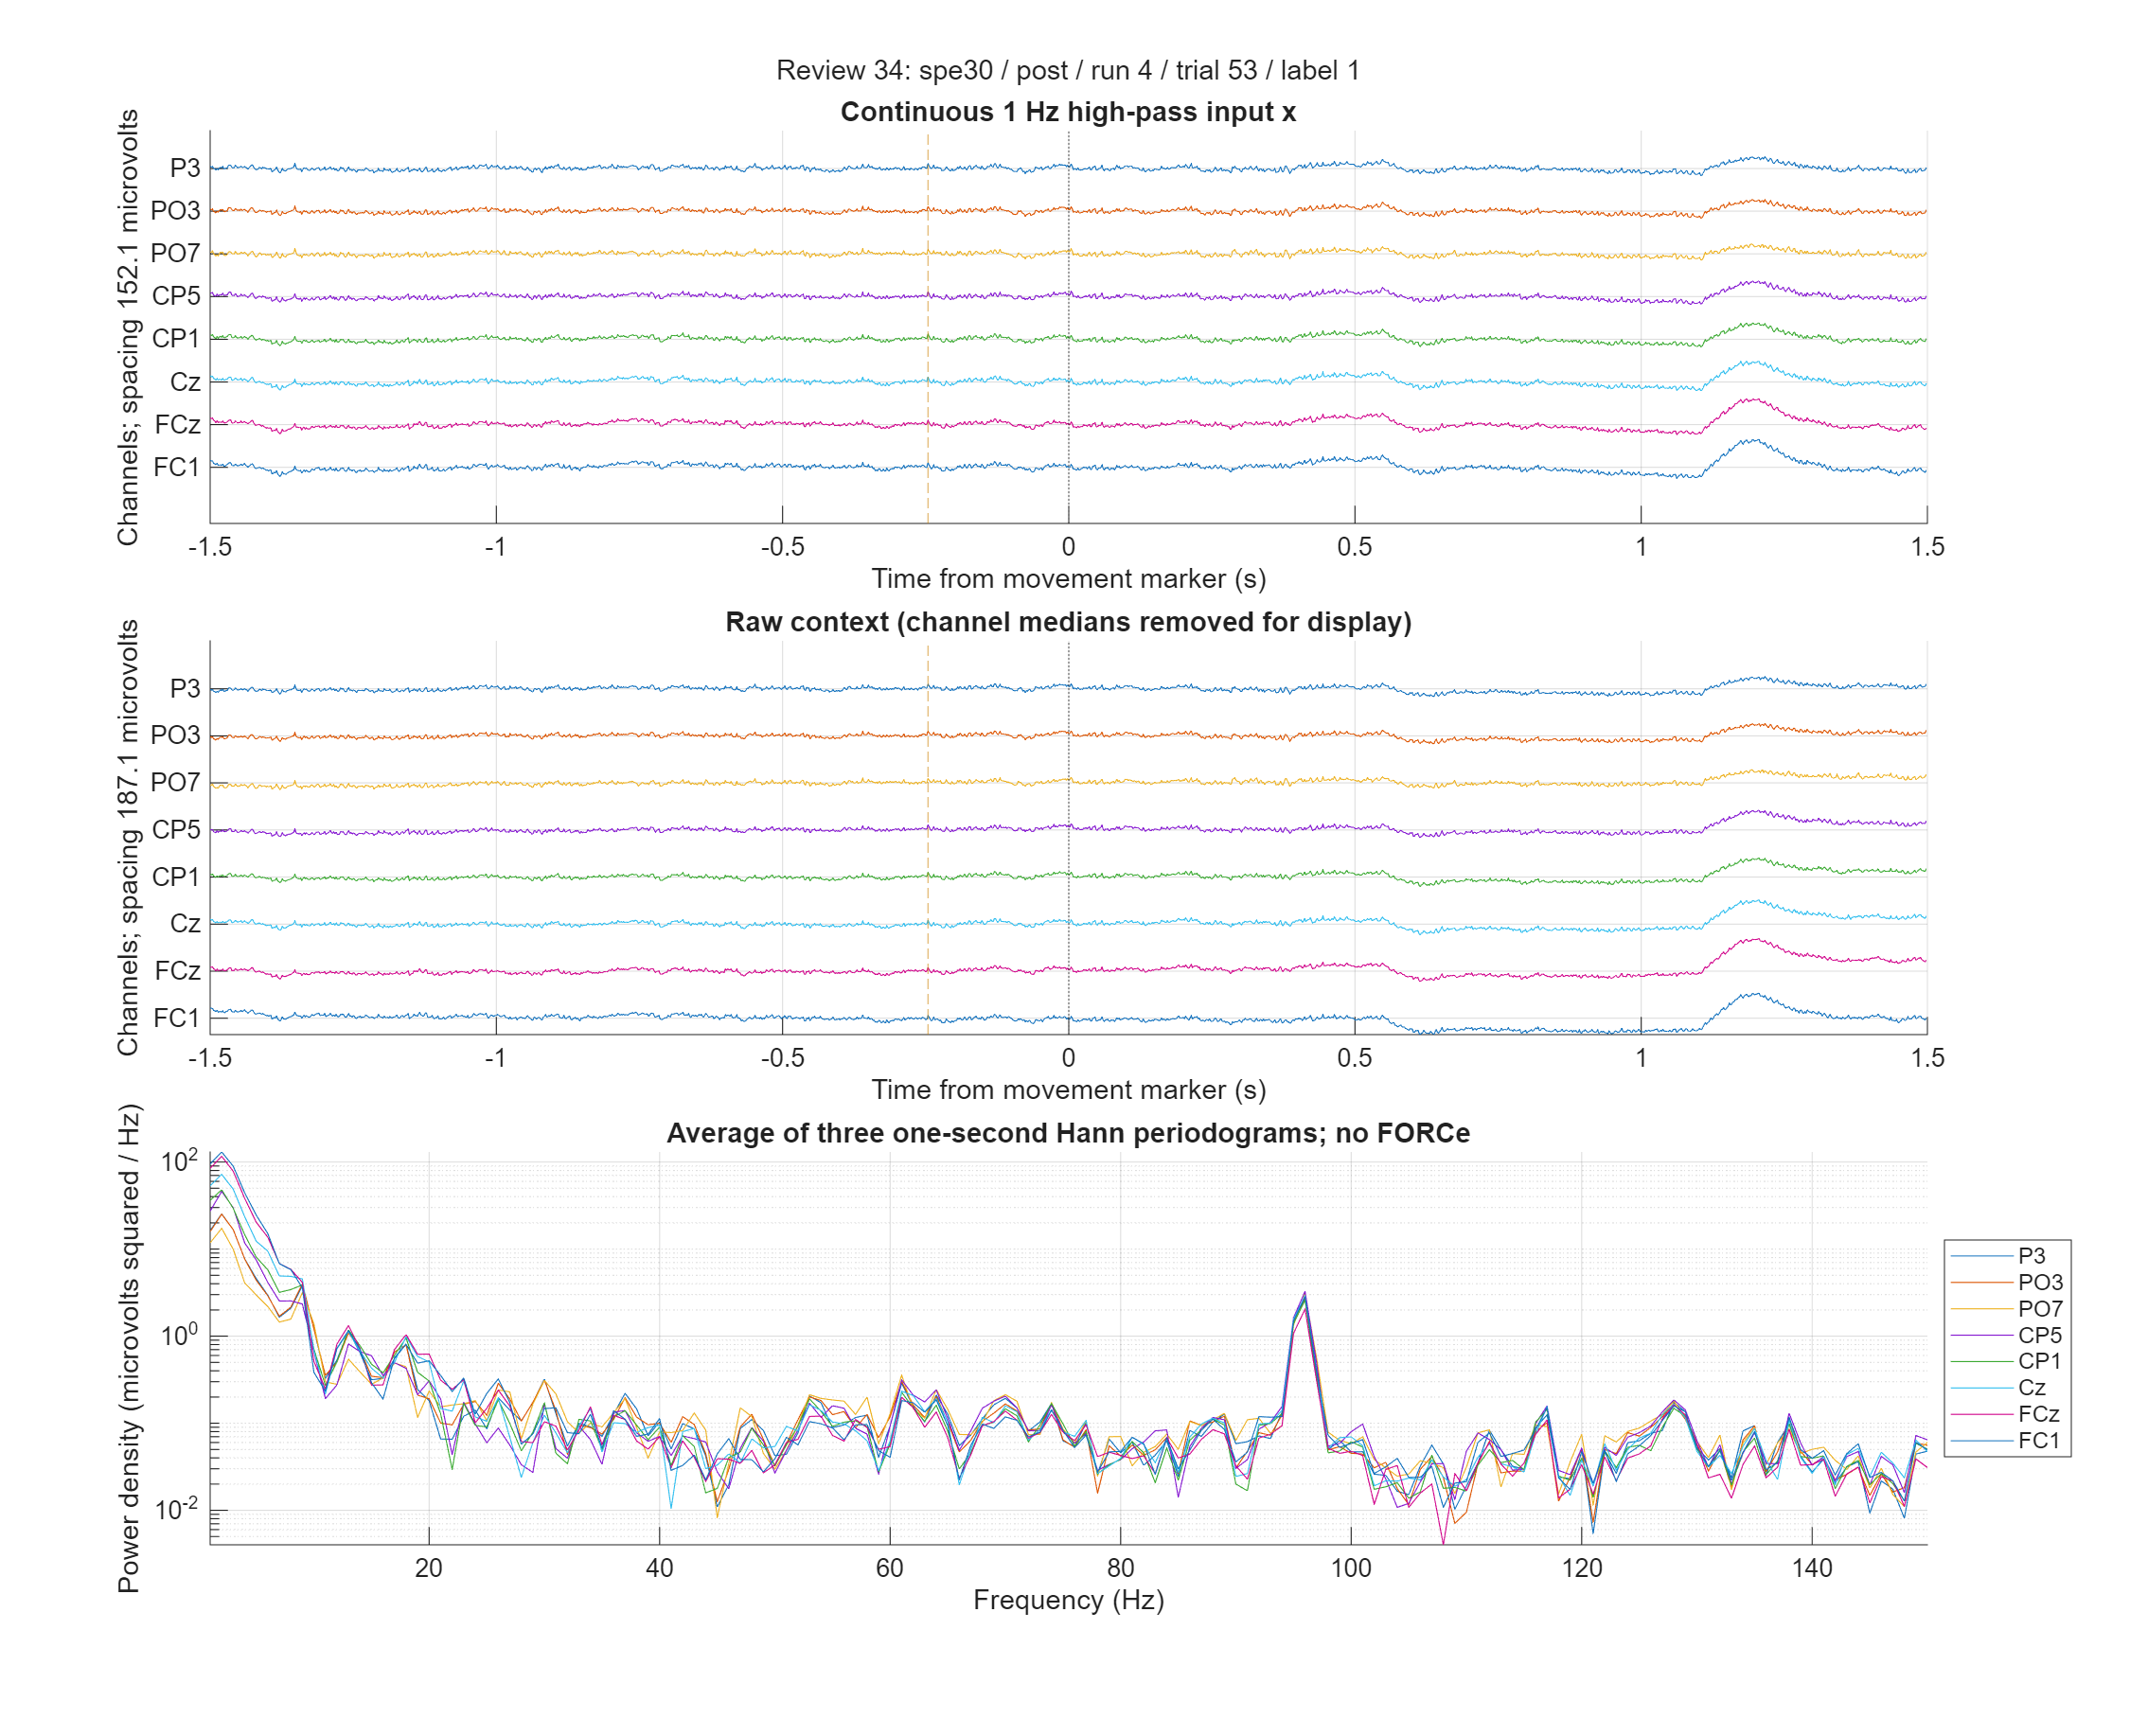
\includegraphics[width=\linewidth,height=.78\textheight,keepaspectratio]{figures/review_034.png}\end{center}\clearpage
\subsection*{Review 35: mle01 / retest / run 3 / trial 62}
\textbf{Selected for suspected contamination: line-frequency content.} Selected without gross excursions above 1 mV. This example is not restricted to the 100 microvolt display stratum.
\begin{center}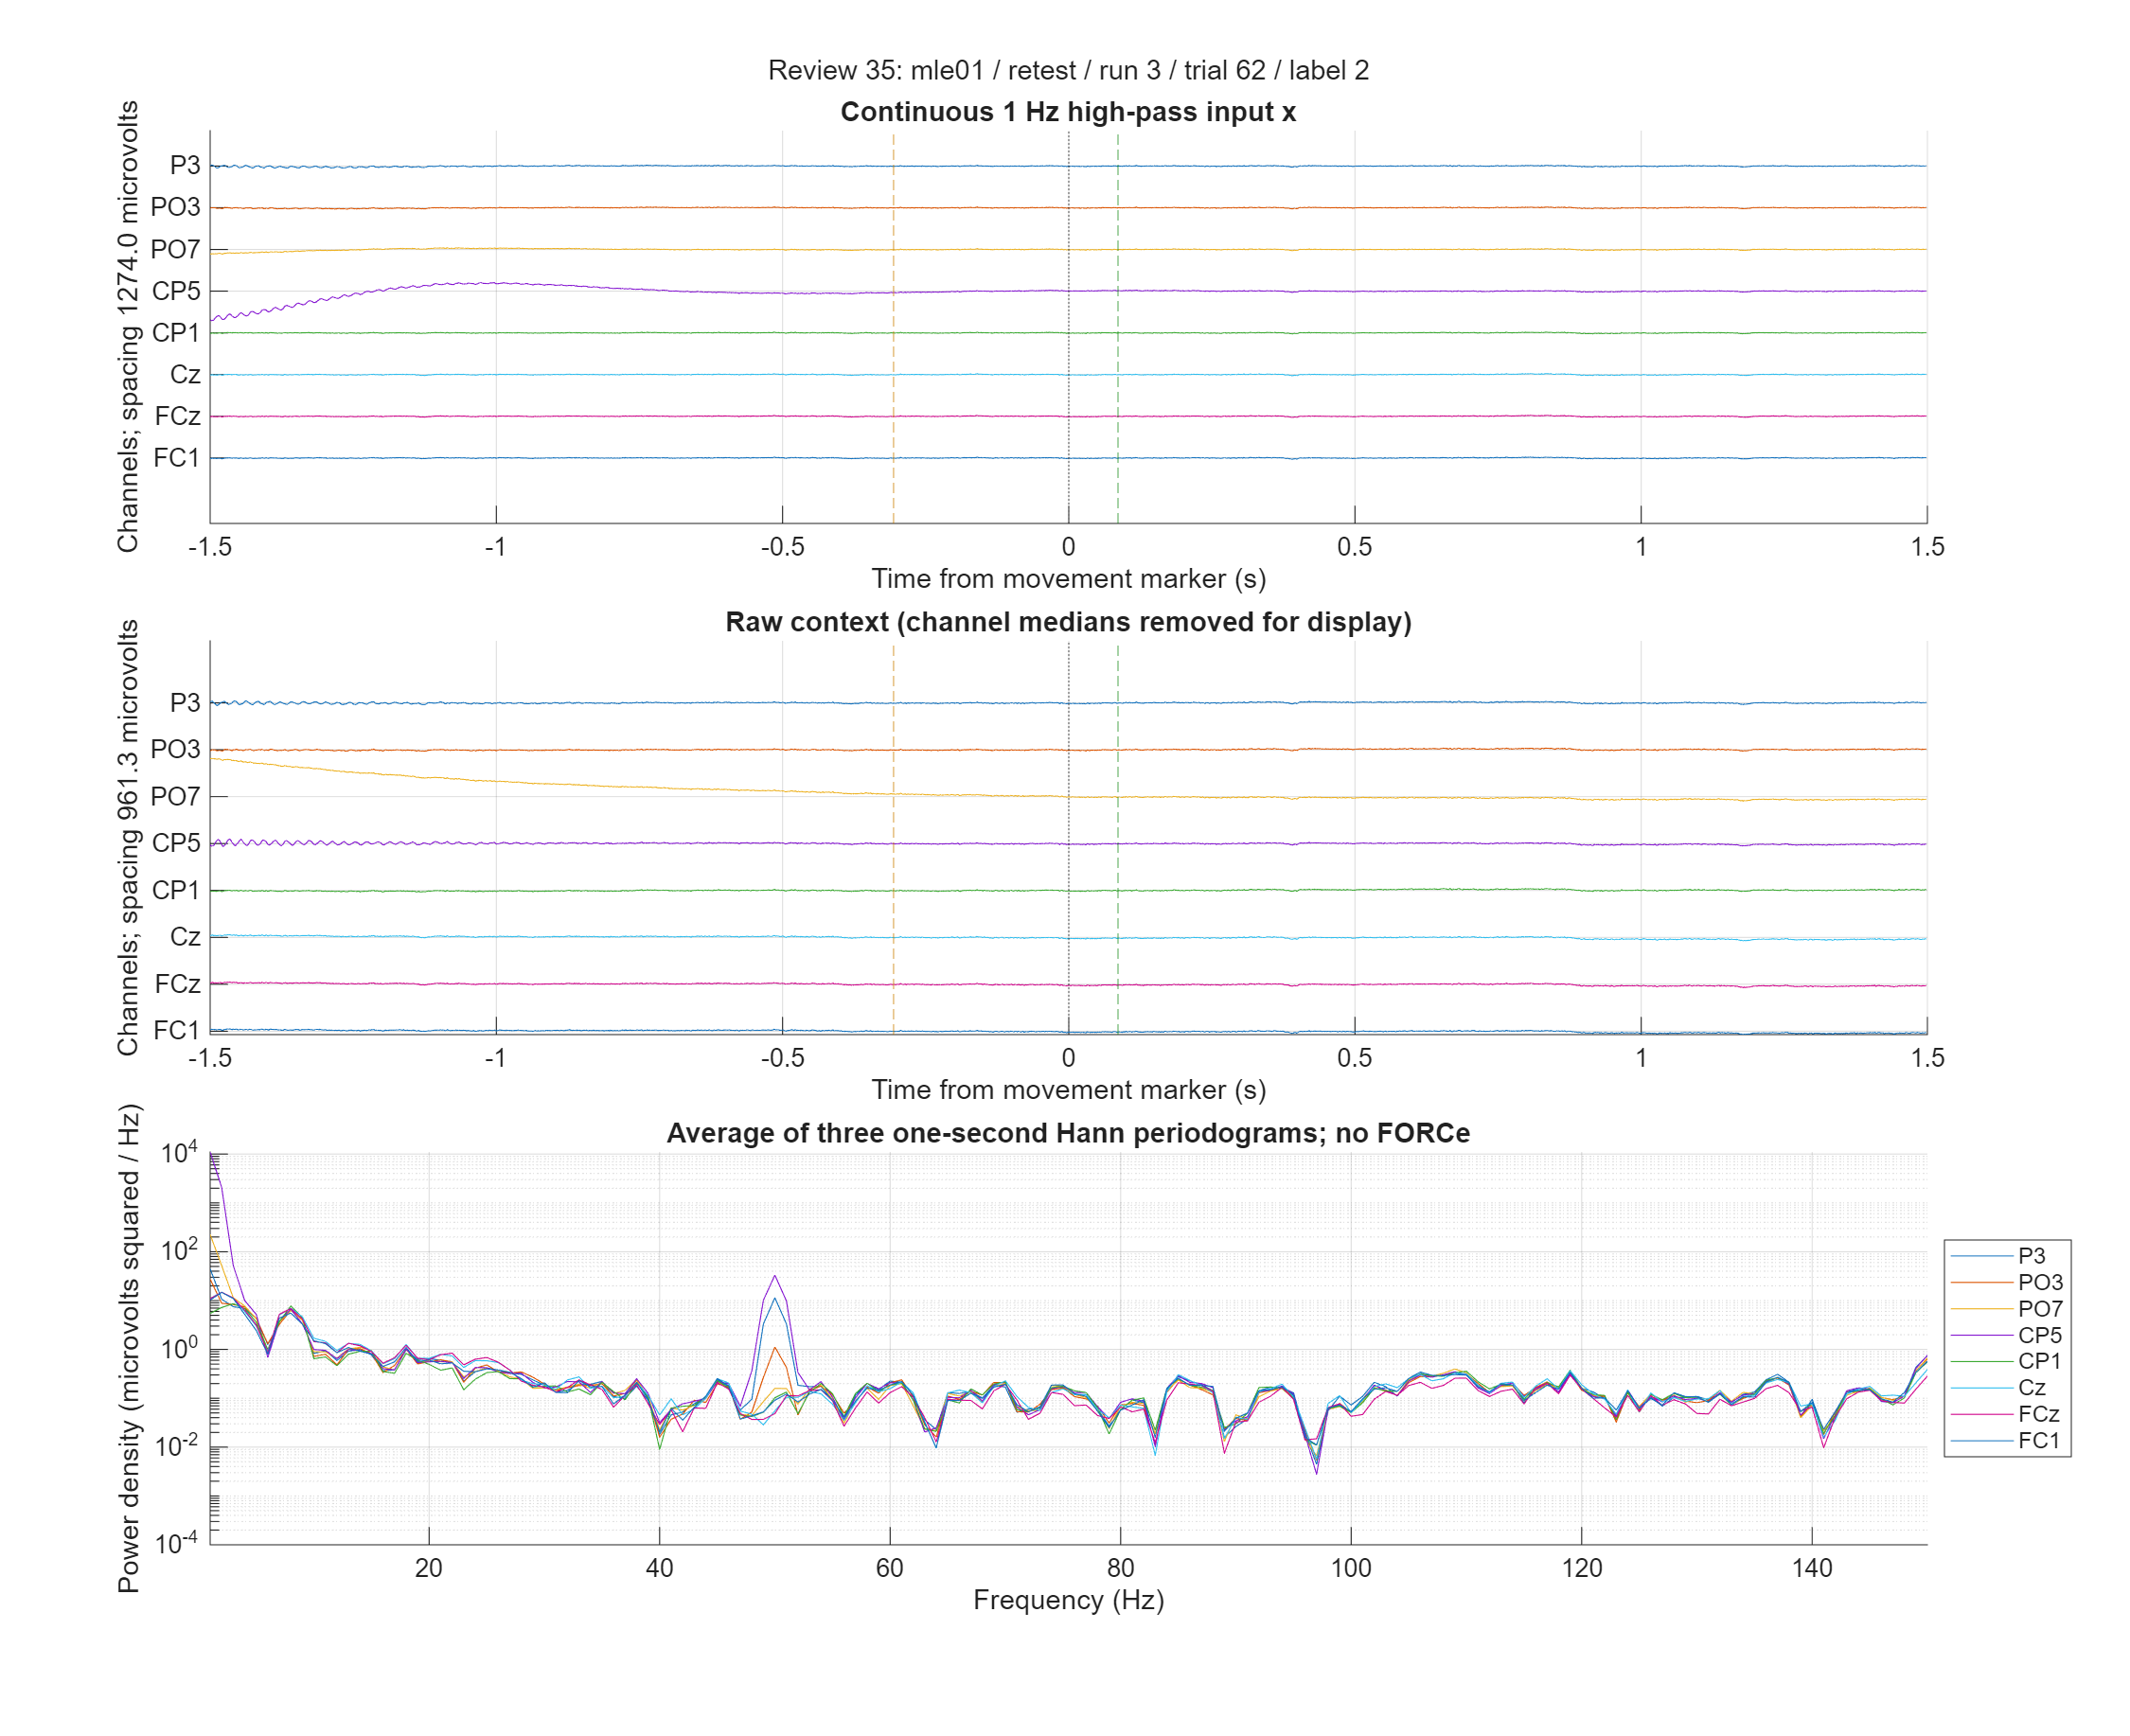
\includegraphics[width=\linewidth,height=.78\textheight,keepaspectratio]{figures/review_035.png}\end{center}\clearpage
\subsection{Event-aligned input context}\label{sec:eventcontext}
\subsubsection*{mle01}
These input means use only the display stratum with whole-interval peak at most 100 \uv. They are not final accepted-trial averages. Posterior traces average PO3/PO7; central traces average Cz/FCz. Movement views use a -0.2 to 0 s baseline; target views use -0.1 to 0 s. ND denotes non-displaced trials and D denotes displaced trials. Plot counts refer to movement averages. Neural source identity remains unresolved.
\begin{center}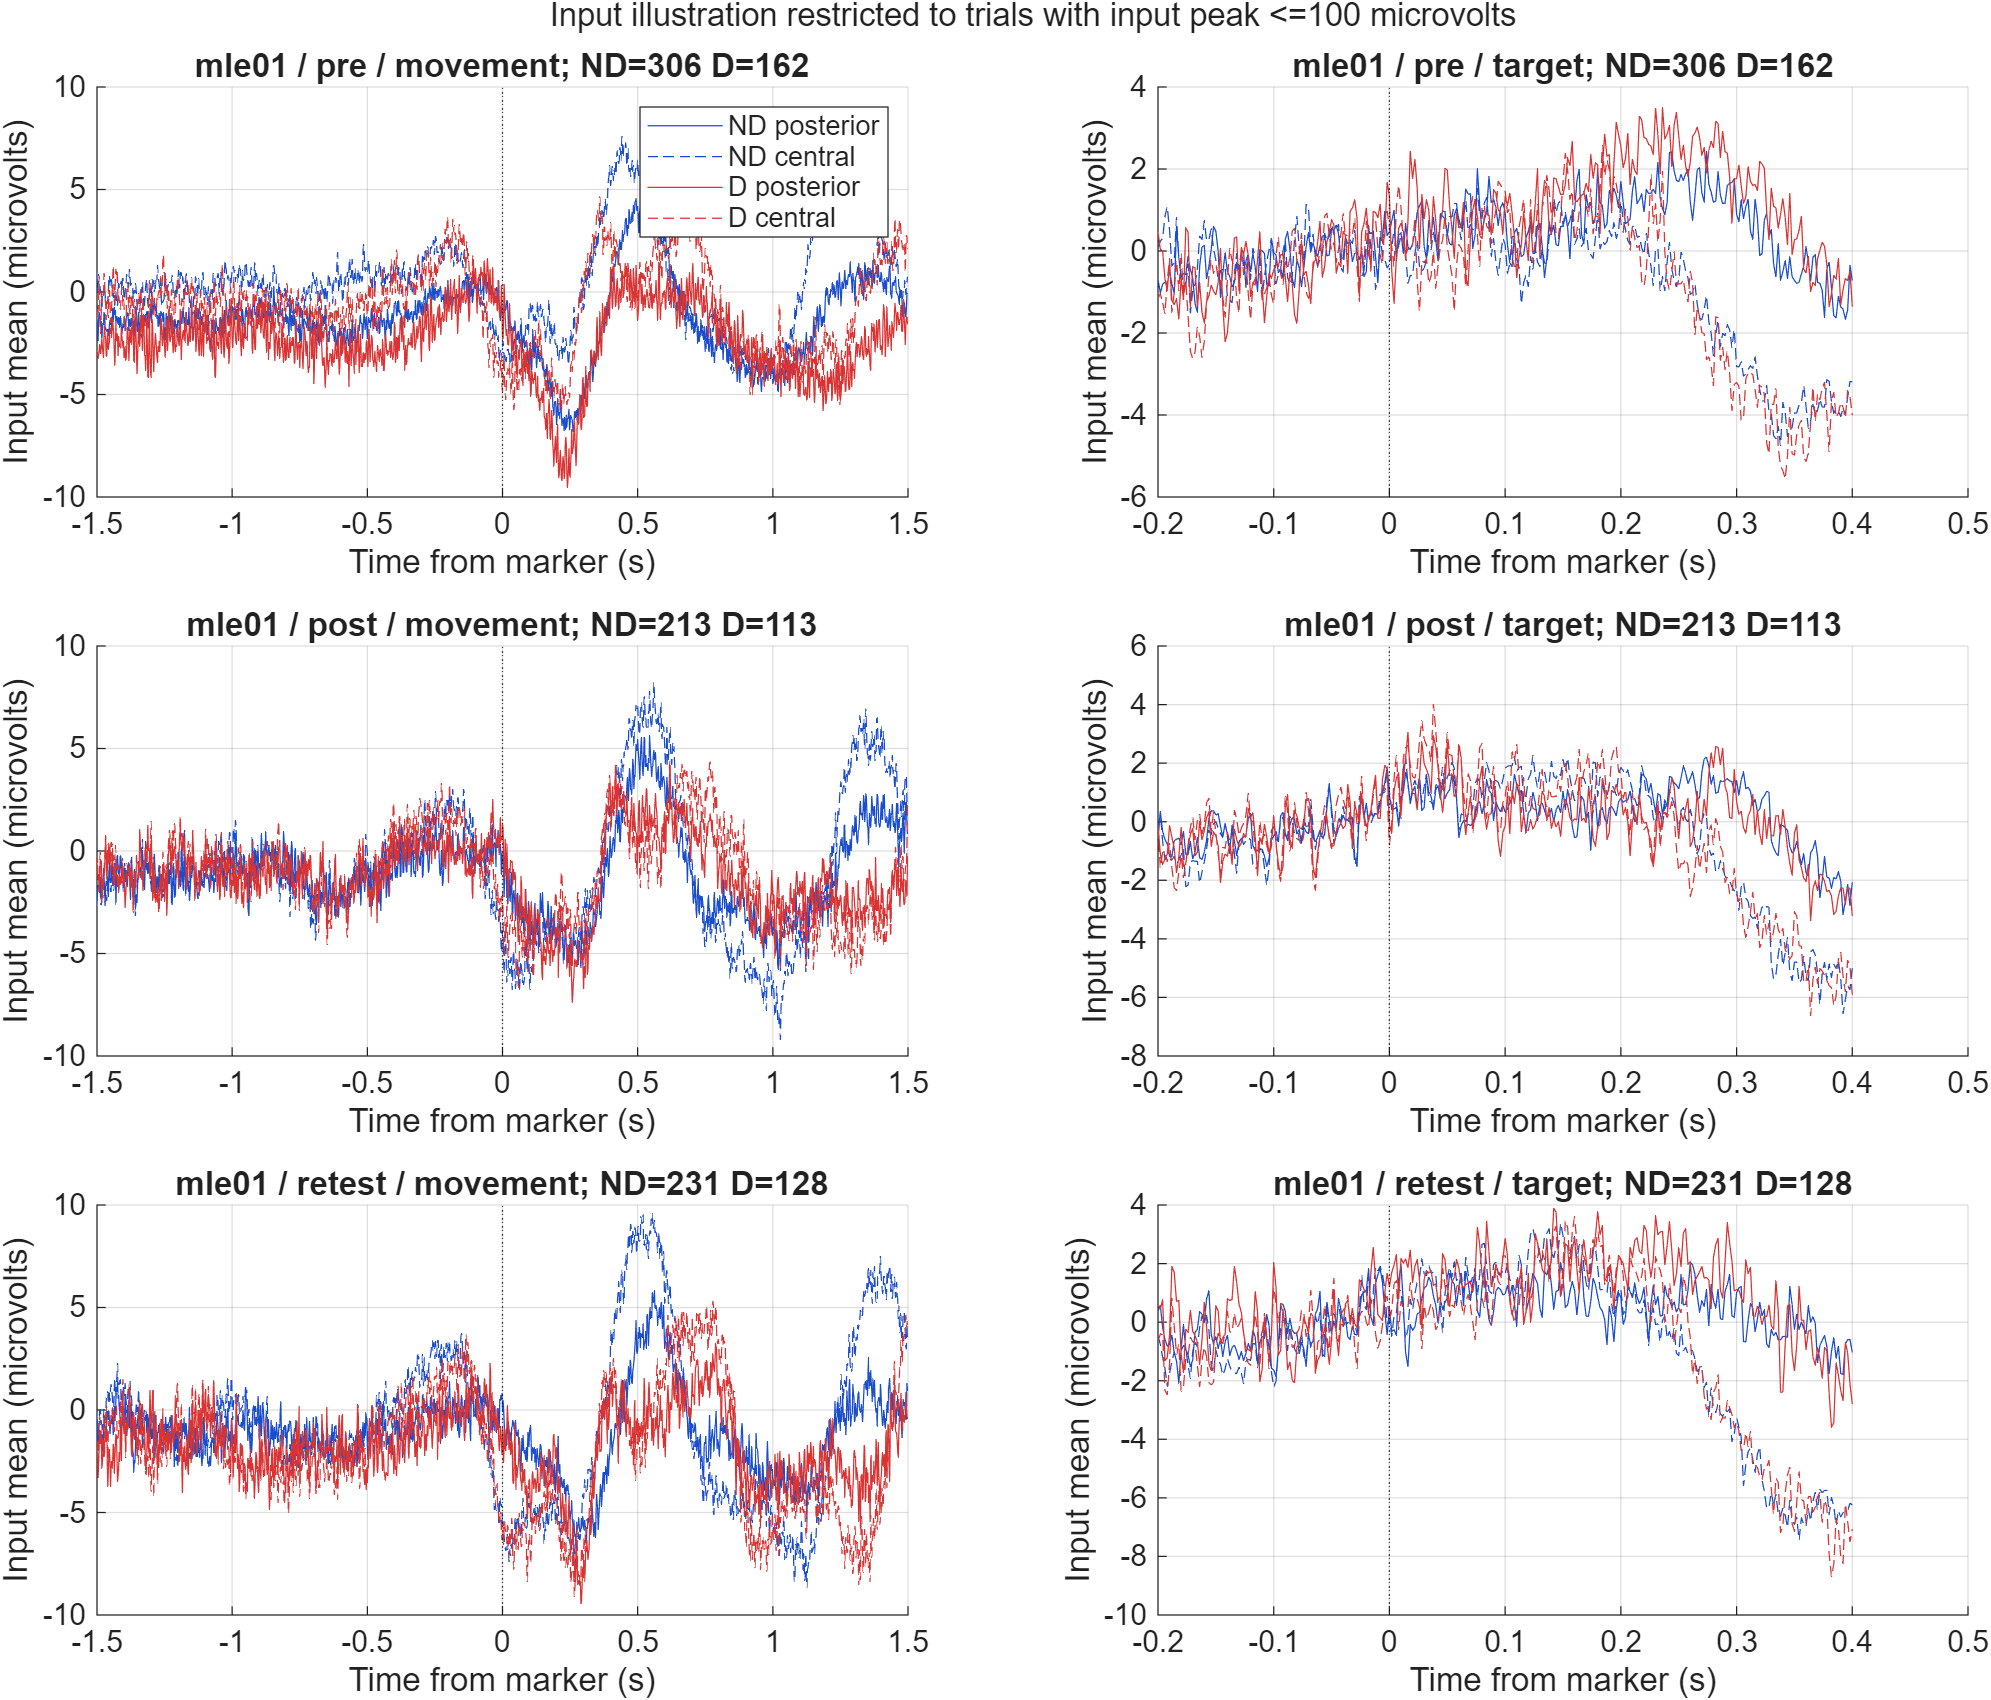
\includegraphics[width=\linewidth,height=.78\textheight,keepaspectratio]{figures/bounded_events_1.png}\end{center}\clearpage
\subsubsection*{spe30}
These input means use only the display stratum with whole-interval peak at most 100 \uv. They are not final accepted-trial averages. Posterior traces average PO3/PO7; central traces average Cz/FCz. Movement views use a -0.2 to 0 s baseline; target views use -0.1 to 0 s. ND denotes non-displaced trials and D denotes displaced trials. Plot counts refer to movement averages. Neural source identity remains unresolved.
\begin{center}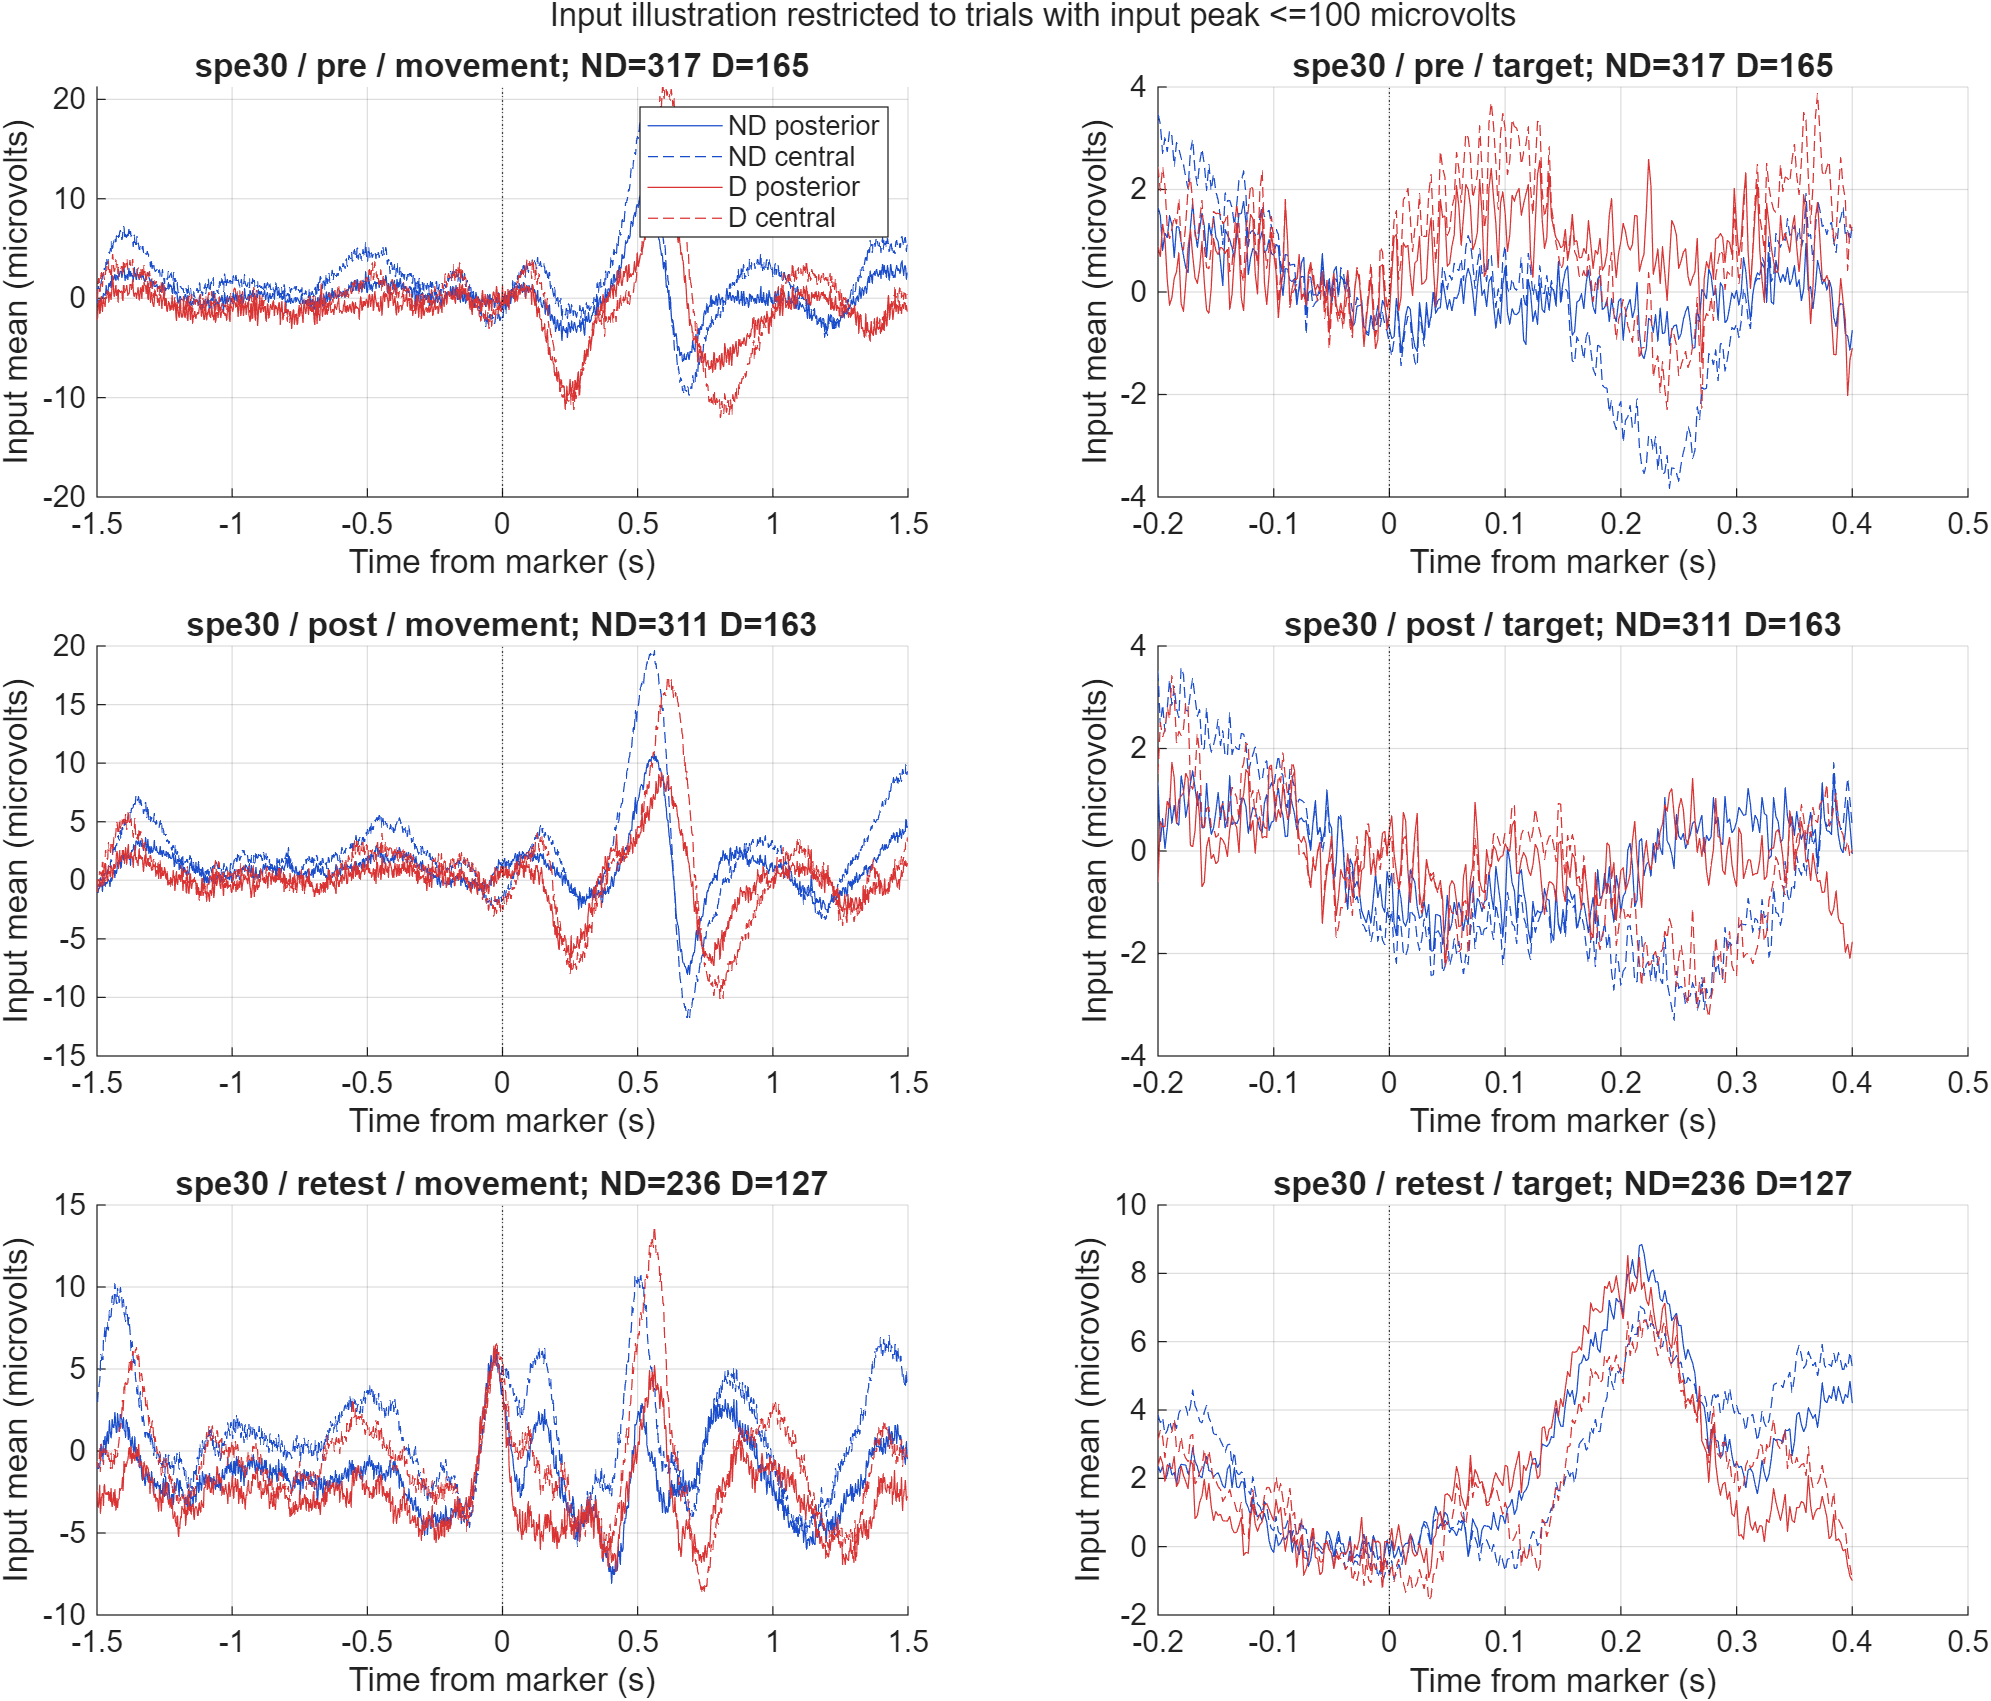
\includegraphics[width=\linewidth,height=.78\textheight,keepaspectratio]{figures/bounded_events_2.png}\end{center}\clearpage
\appendix\section{References}
\begin{thebibliography}{9}
\bibitem{nist} NIST/SEMATECH. \textit{e-Handbook of Statistical Methods}, Section 1.3.5.17: Detection of Outliers. \url{https://www.itl.nist.gov/div898/handbook/eda/section3/eda35h.htm}.
\bibitem{whitham} Whitham et al. (2007). Scalp electrical recording during paralysis: quantitative evidence that EEG frequencies above 20 Hz are contaminated by EMG. \textit{Clinical Neurophysiology}. DOI: \href{https://doi.org/10.1016/j.clinph.2007.04.027}{10.1016/j.clinph.2007.04.027}.
\bibitem{plochl} Pl\"ochl, Ossand\'on and K\"onig (2012). Combining EEG and eye tracking: identification, characterization, and correction of eye movement artifacts in electroencephalographic data. \textit{Frontiers in Human Neuroscience}. DOI: \href{https://doi.org/10.3389/fnhum.2012.00278}{10.3389/fnhum.2012.00278}.
\bibitem{graz} Amaunam et al. (2024). EEG correlates of error-related activity during ballistic computer mouse movements. 9th Graz BCI Conference.
\end{thebibliography}
\section{Review and reproducibility materials}
The accompanying inventory records every eligible trial and all channel-window measurements. The review set contains 29 run-stratified representative inputs and six enriched examples. Informal expert comments can be recorded in Section~\ref{sec:review}; systematic source annotations have not been collected. All numerical screens are reproducible from the saved input-screen script; the report does not modify the production pipeline or previously saved results.
\end{document}
